\label{sec:vbf-nonres}
\subsubsection{Non-resonant \Mbb{} distribution}
In order to determine the non-resonant background, we fit  the sidebands of each of the BDT regions independently with an analytical function. An alternative approach  using a control region and a linear transfer factor to relate the control region shape to the signal regions is documented in Appendix~\ref{sec:vbf-app-oldfitbkgds}.  However, due to concerns about the validity of the approach, documented in Appendix~\ref{sec:vbf-app-LinearityTest}, the more conservative approach of independent fits is taken here.  

The sidebands of the \Mbb{}  distribution of each BDT region are shown in Fig. \ref{fig:vbf-mbb_sidebands}.

\begin{figure}[htbp]
  \centering
 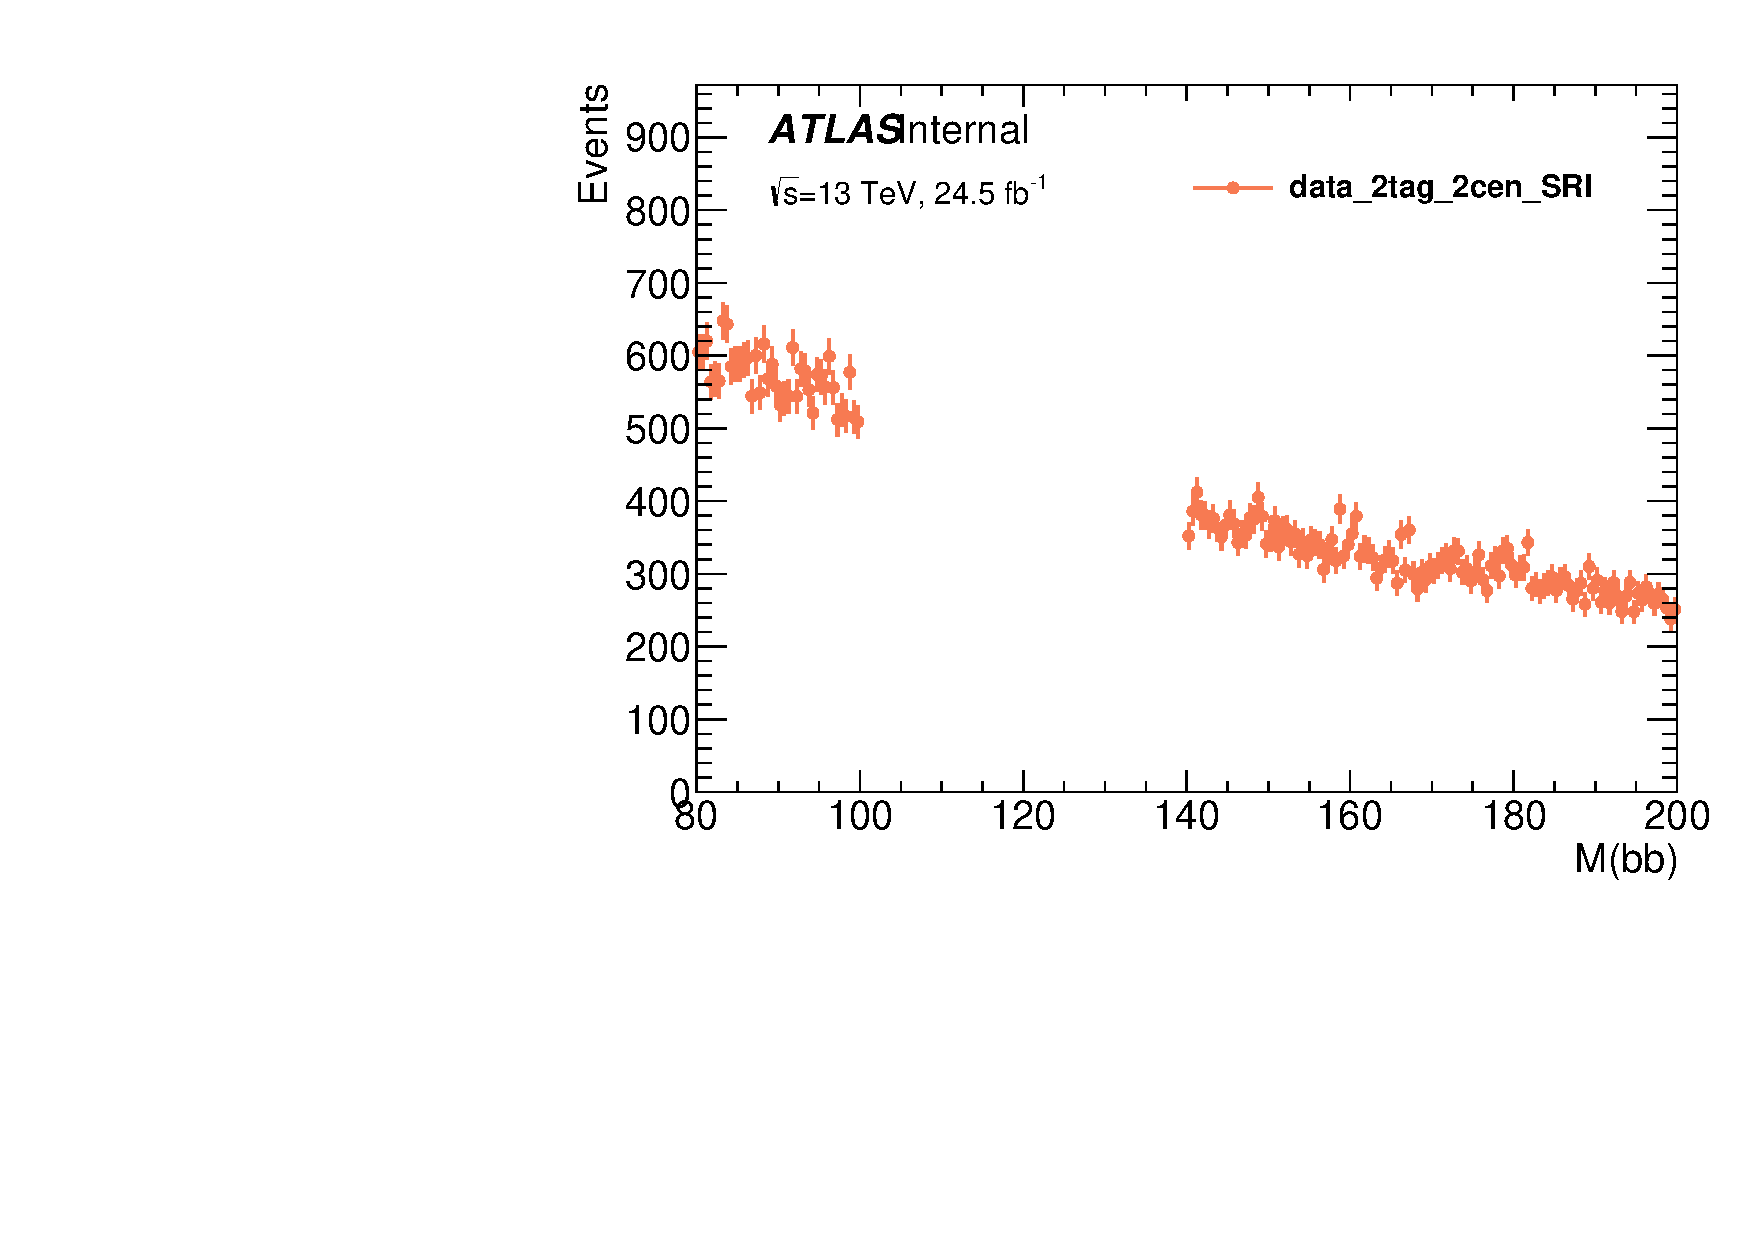
\includegraphics[width=0.45\textwidth]{figures/VBF/Mbb_SRI_2cen.pdf}
 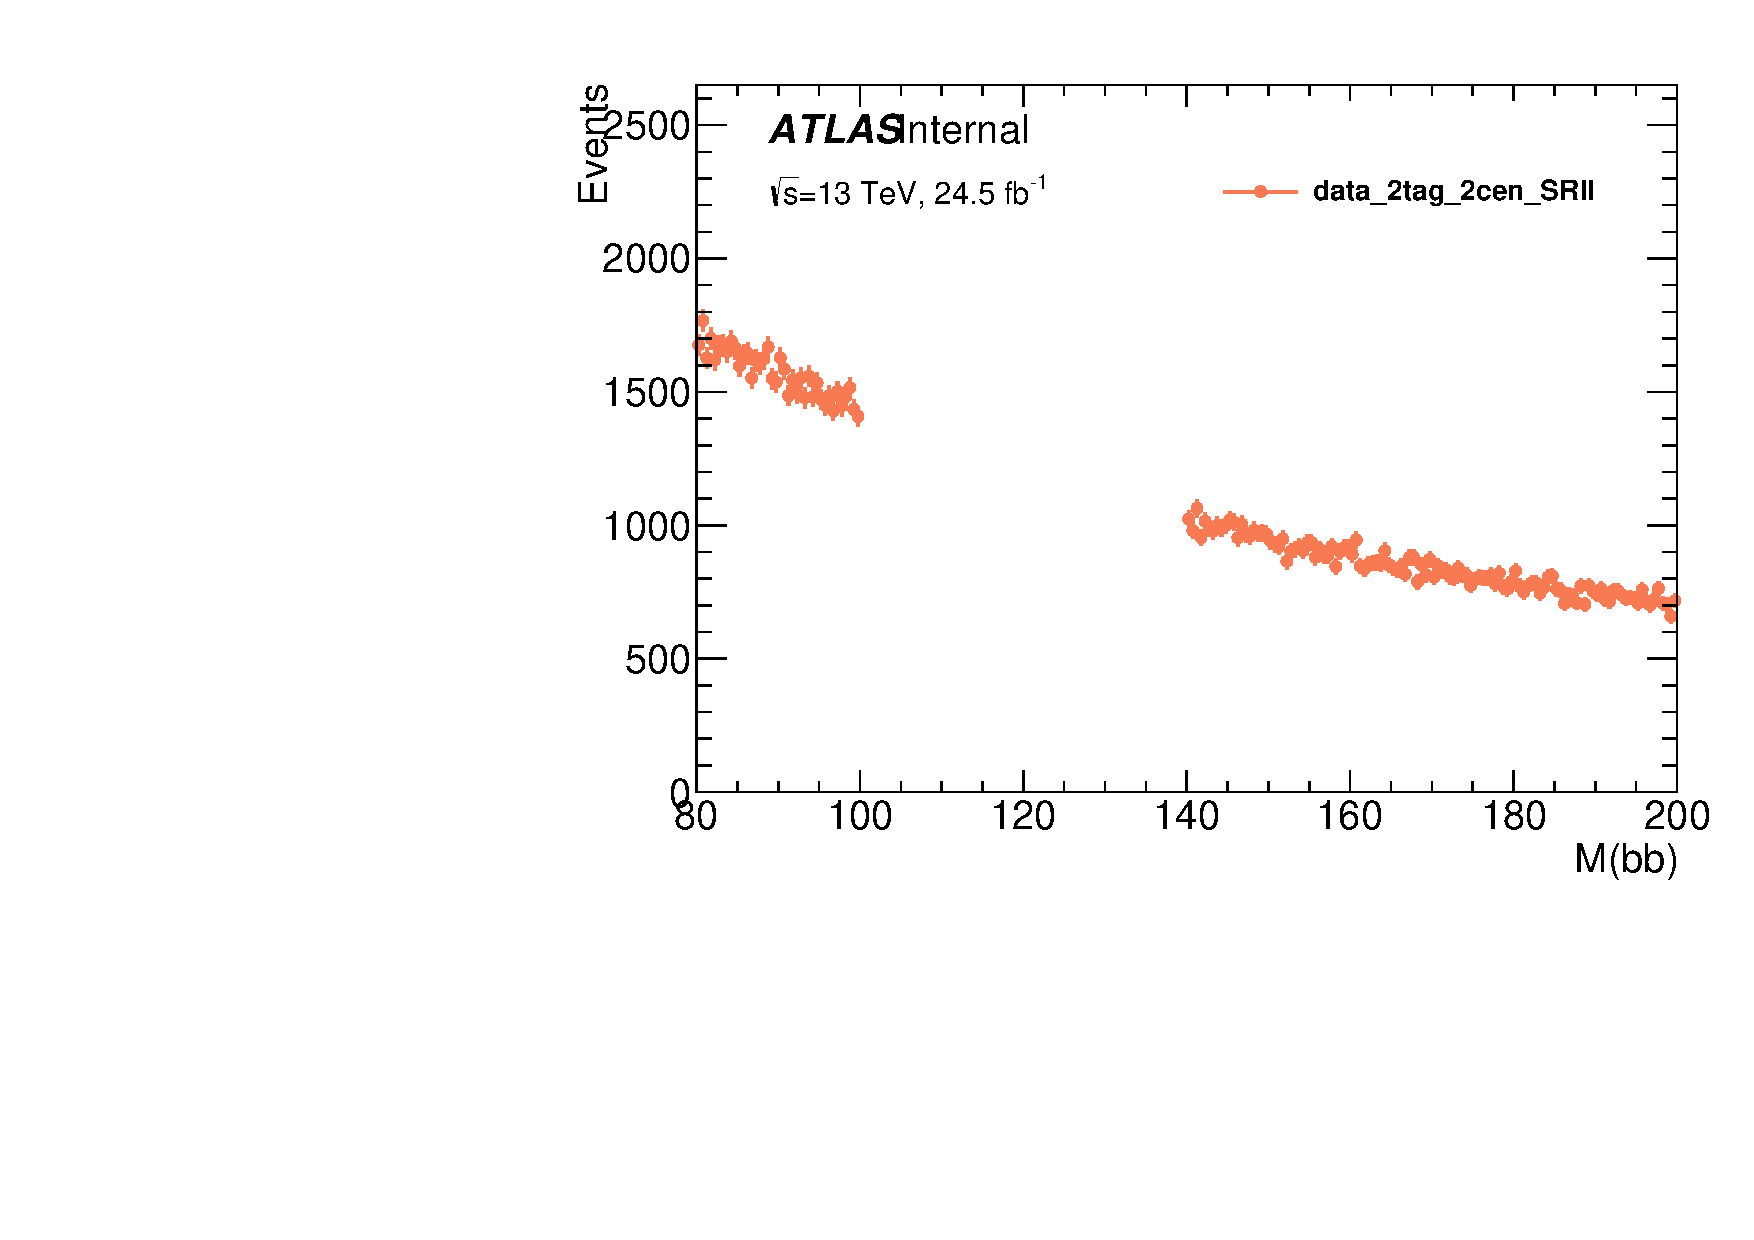
\includegraphics[width=0.45\textwidth]{figures/VBF/Mbb_SRII_2cen.pdf}\\
 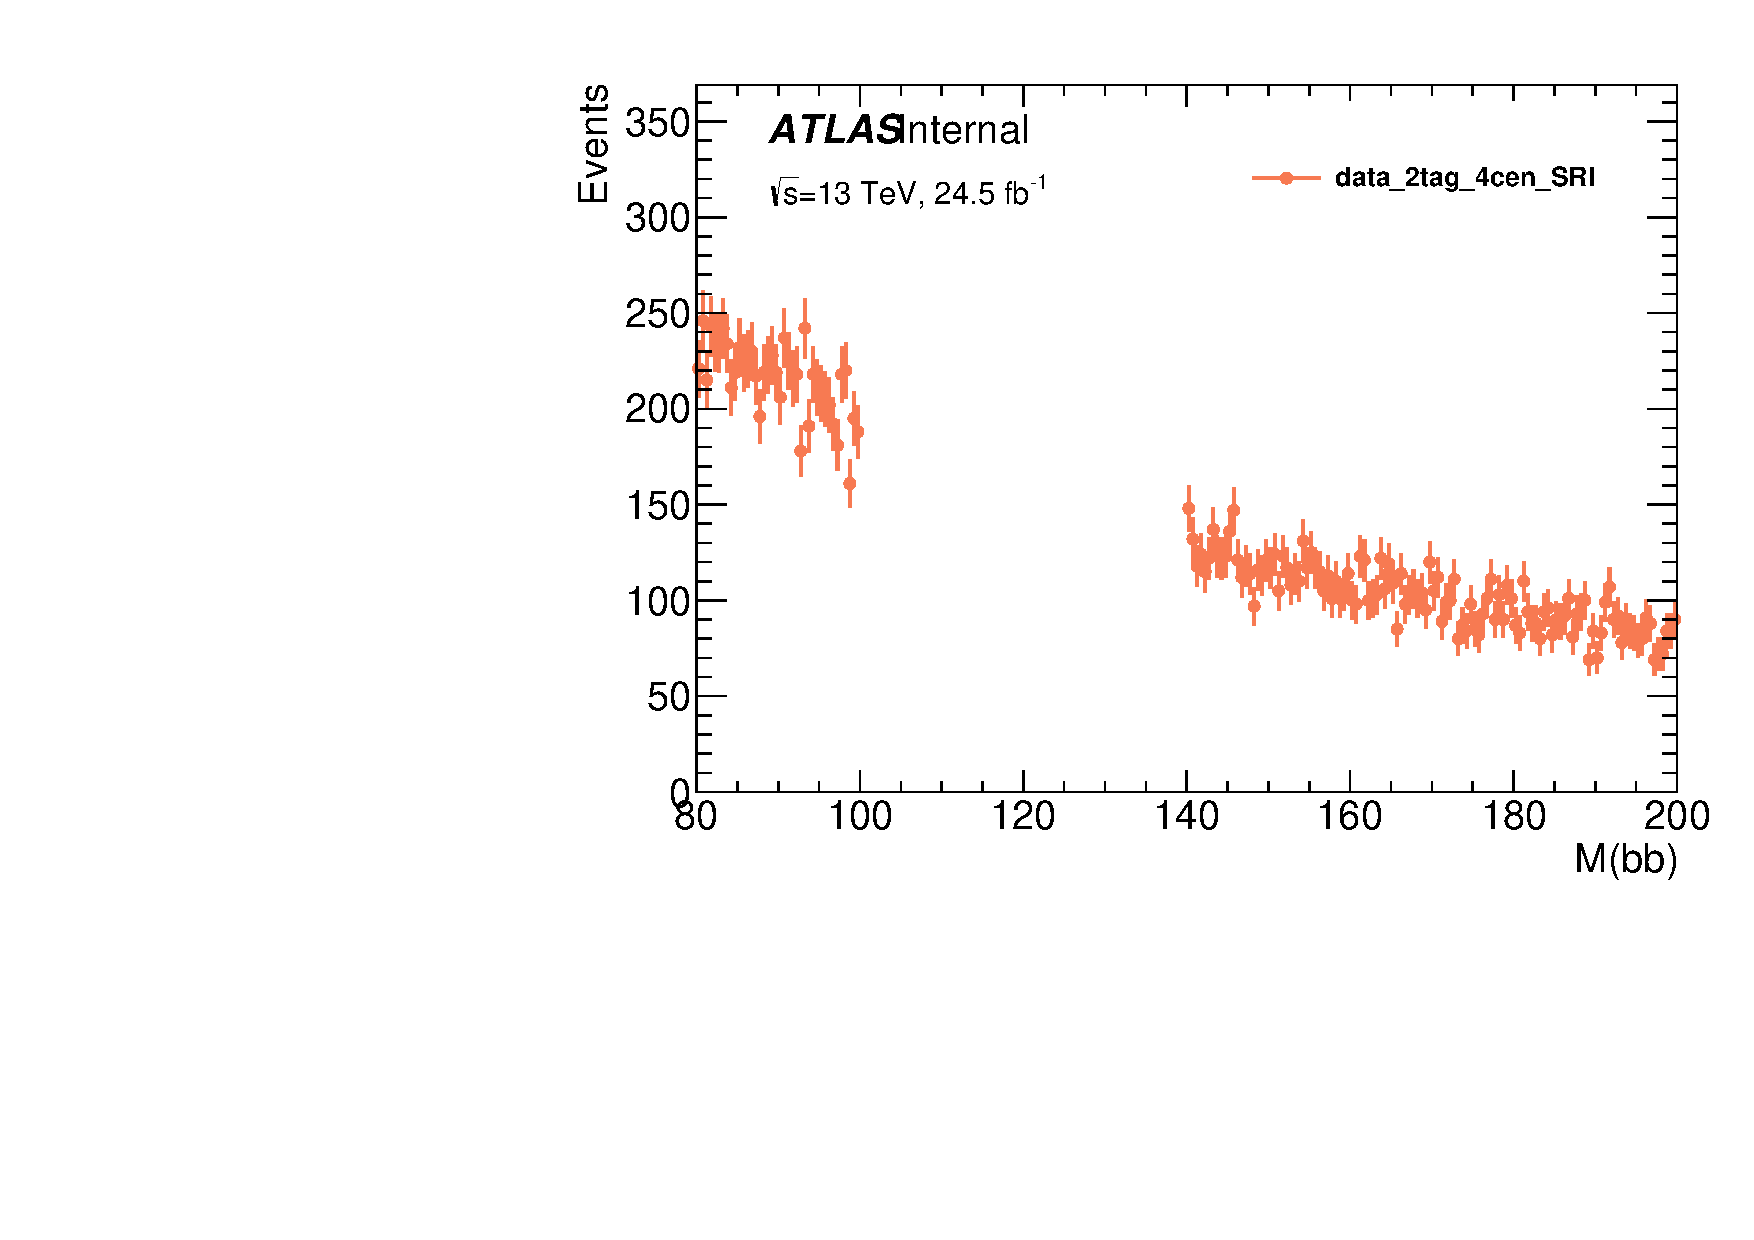
\includegraphics[width=0.45\textwidth]{figures/VBF/Mbb_SRI_4cen.pdf}
 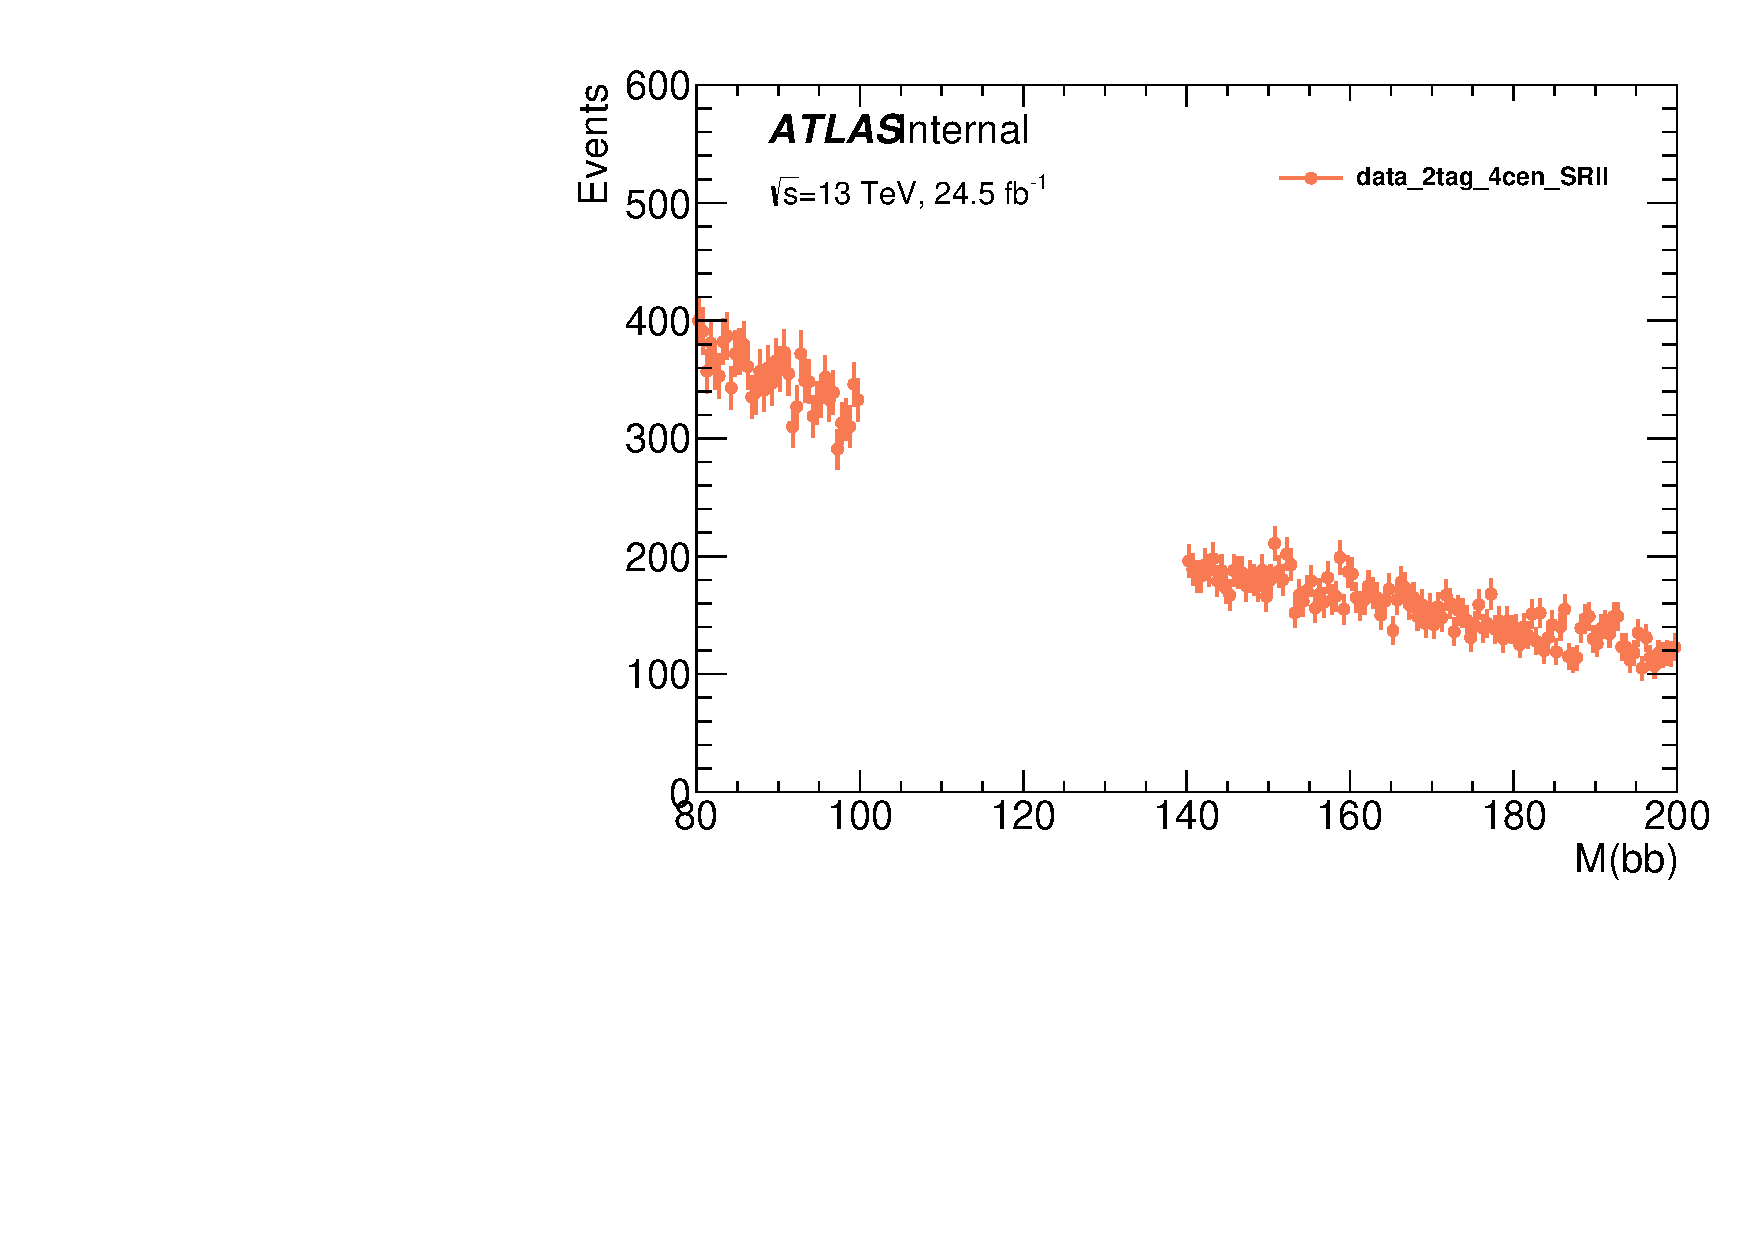
\includegraphics[width=0.45\textwidth]{figures/VBF/Mbb_SRII_4cen.pdf}\\
 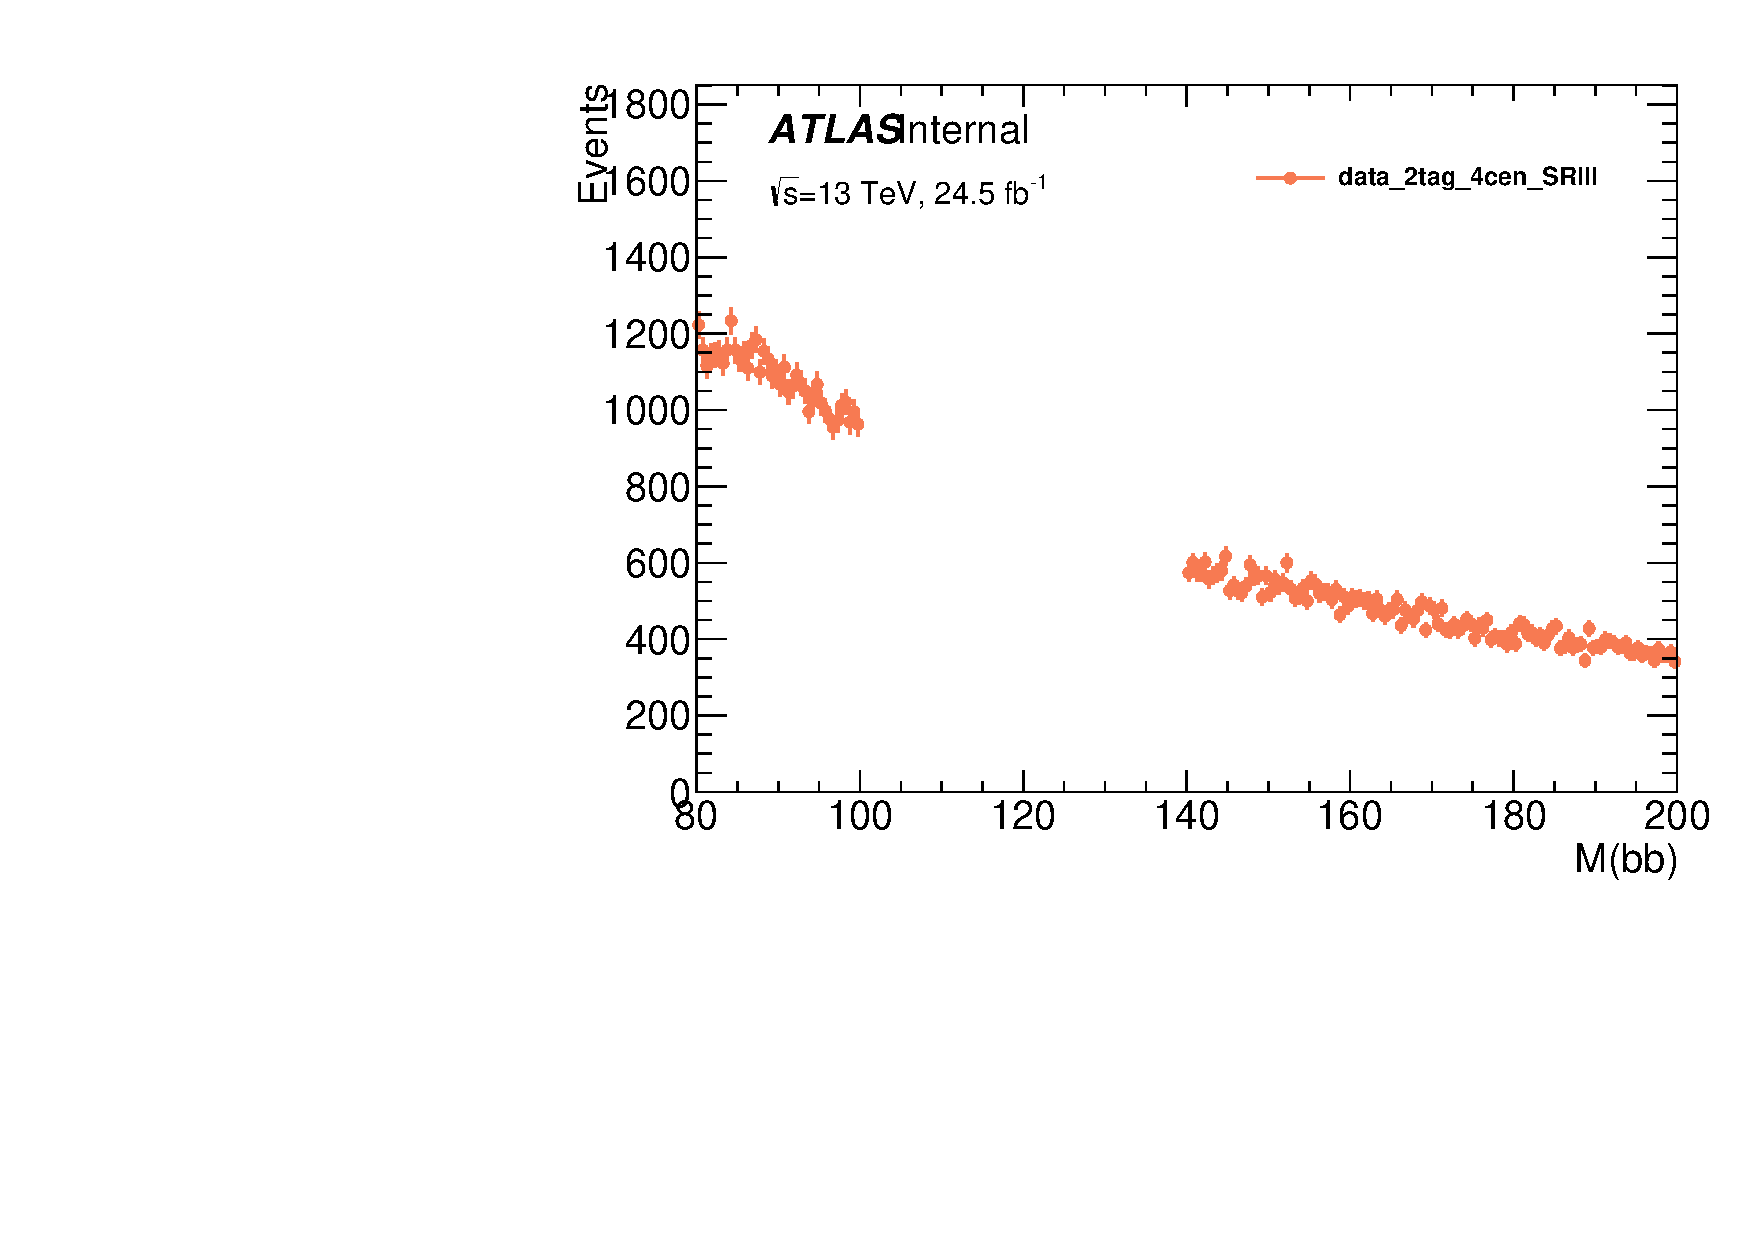
\includegraphics[width=0.45\textwidth]{figures/VBF/Mbb_SRIII_4cen.pdf}
 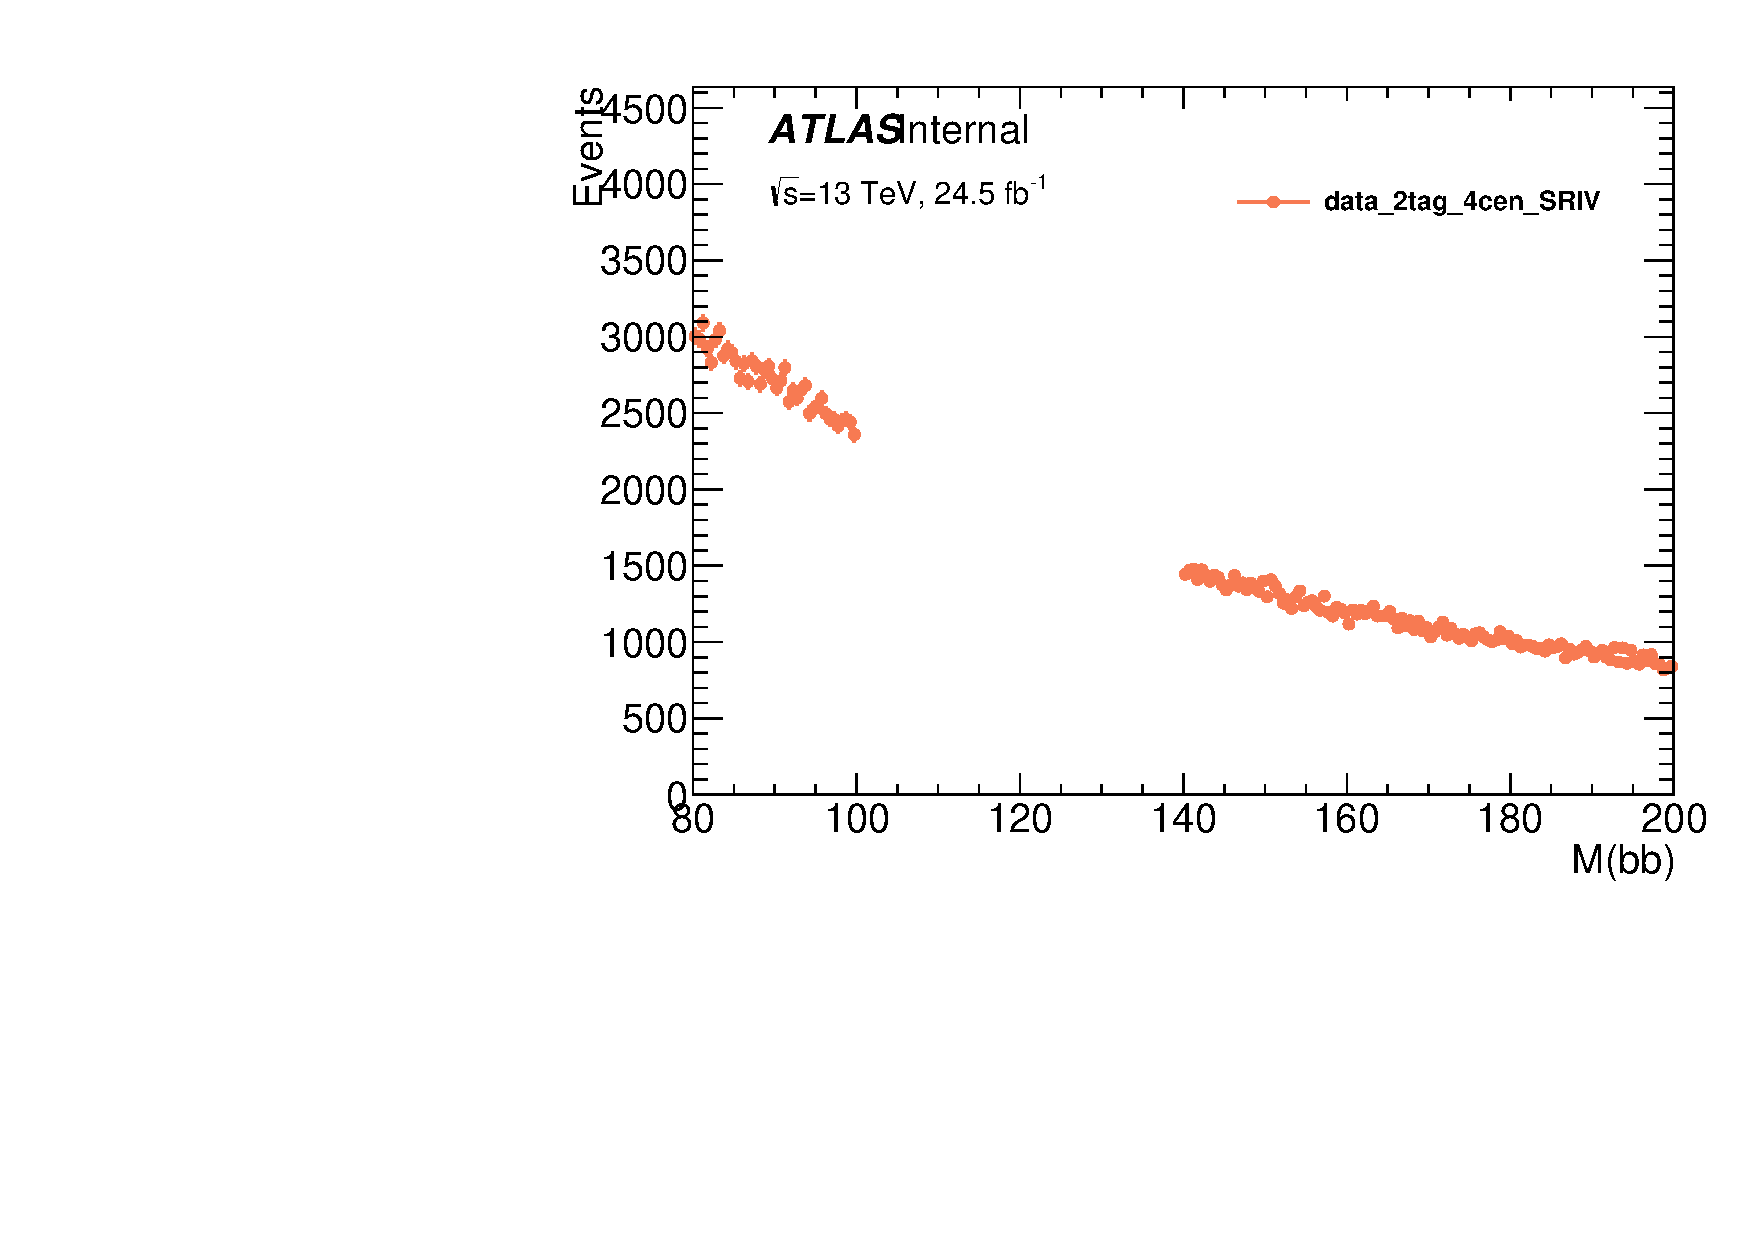
\includegraphics[width=0.45\textwidth]{figures/VBF/Mbb_SRIV_4cen.pdf}\\
\caption{\Mbb{} shapes of all BDT regions in sidebands} 
  \label{fig:vbf-mbb_sidebands}
\end{figure}



\paragraph{Function choice}

Several functions are considered and tested. The functions are required to pass two conditions:

\begin{itemize}
\item 
Compatibility: The function must be statistically  compatible with the sidebands of the \Mbb{} distribution in the signal regions, where the Higgs mass range $100<\Mbb<140$ GeV is ignored. The compatibility criterion is defined as $P(\chi^2)>0.05$ and $P(F-\rm{test})>0.05$,  where the $\chi^2$ and $F-\rm{test}$ probabilities are considered, respectively. The $F-\rm{test}$ is performed with respect to the $n+1$ order function.  Only statistical errors are considered in these fits.  Among the candidates satisfying the conditions above, the function with the smallest number of degrees of freedom is chosen. For this study, the \zjets{} component is included in the fit,  normalized to the SM prediction.


\item Spurious Signal:  The lowest order function that satisfies compatibility condition, $f_{B}$, is tested against the the lowest order functions in an alternative truth model, $f_{A}$, that also satisfies the compatibility condition, to derive the spurious signal size \cite{CMS-HIG-12-028}.  We build pseudo data from $f_{A}$, where the parameters of the function are derived from the fit to the sidebands in each signal region.  We then fit the distribution with $f_{B}$ plus $\mu_{sp}$ times the signal template. The measured  apparent signal size needs to be less than $50\%$ of the actual signal size. If this test fails, the the next order function satisfying the compatibility condition is tested.  The \zjets{} component is not included in the pseudo data.

\end{itemize}

 Among the candidates satisfying the conditions above, the function with the smallest
number of degrees of freedom is chosen.


The family of functions considered is that of the Bernstein polynomials listed in Equation~\ref{eq:bernstein}, which were
used successfully in the previous iteration of this analysis.  The product of Bernstein and exponential functions, as well as the sum of exponentials, were used as the alternative truth functions. 

\begin{equation}
\label{eq:bernstein}
\begin{aligned}
\textnormal{Berstein O2} &= a_1(1-k)^2 + 2a_2(1-k)k + a_3k^2, \\
\textnormal{Berstein O3} &= a_1(1-k)^3 + 3a_2(1-k)^2k + 3a_3(1-k)k^2 + a_4k^3, \\
\textnormal{Berstein O4} &= a_1(1-k)^4 + 4a_2(1-k)^3k + 6a_3(1-k)^2k^2 + 4a_4(1-k)k^3 + a_5k^4,\\
\textnormal{Berstein O5} &= a_1(1-k)^5 + 5a_2(1-k)^4k + 10a_3(1-k)^3k^2 + 10a_4(1-k)^2k^3 + 5a_5(1-k)k^4 +a_6k^5, \\
\textnormal{where } k &\equiv \frac{(x-80)}{120}
\end{aligned}
\end{equation}


The $\chi^2$ values and probabilities and $F-\rm{test}$ probabilities are summarized in Tables~\ref{tab:chi2-2cen} through~\ref{tab:f-test}. The $\chi^2$ test criteria are met for the O(2) Bernstein function in all regions, except in 
SR IV of the \fourcentral channel where we need at least an O(3) Bernstein function. The $F$-test is passed for functions which pass the $\chi^2$ criterion in all channels and regions.

The spurious signal fits are given in Tables~\ref{tab:spurious-test-2cen} and~\ref{tab:spurious-test-4cen}, which additionally show which functions are used as the alternative truth models.  The spurious Asimov fit plots are shown in Figures \ref{fig:vbf-Fit_SP_2cen} and \ref{fig:vbf-Fit_SP_4cen}. In most regions the O(3) Bernstein polynomial satisfies the spurious signal criterion. Note that our choice of background function minimizes the potential bias in trade of variance, i.e. the higher order functional forms yield larger uncertainty as shown in Table. \ref{tab:perchannel_sensitivity}.

To satisfy all of the criteria, we choose an O(3) Bernstein function for the \twocentral channels, as well as for all SR of the \fourcentral channel except SRIV which uses O(4).  


\begin{table}[htbp]
\centering
\caption{Background only fit $\chi^2$ and Prob($\chi^2$) for \twocentral region. The first number in each cell is the $\chi^2$ and the number in parentheses is the probability.}
\label{tab:chi2-2cen}
\begin{tabular}{|l|l|l|l|l|l|l|}
\hline
   & \multicolumn{3}{c|}{\twocentral SR I}      & \multicolumn{3}{c|}{\twocentral SR II}     \\ \hline
   & Bernstein   & Expo*Bernstein & Sum of Expo & Bernstein   & Expo*Bernstein & Sum of Expo \\ \hline
O2 & 1.08 (0.23) & 1.08 (0.22)    & 1.13 (0.13) & 0.87 (0.88) & 0.84 (0.92)    & 0.84 (0.92) \\ \hline
O3 & 1.08 (0.22) & 1.07 (0.24)    & 1.19 (0.19) & 0.85 (0.92) & 0.85 (0.91)    & 0.85 (0.91) \\ \hline
O4 & 1.07 (0.27) & 1.07 (0.25)    & 1.11 (0.16) & 0.85 (0.92) & 0.85 (0.91)    & 0.87 (0.88) \\ \hline
O5 & 1.07 (0.27) &                &             & 0.85 (0.92) &                &             \\ \hline
\end{tabular}
\end{table}


\begin{table}[htbp]
\centering
\caption{Background only fit $\chi^2$ and Prob($\chi^2$) for \fourcentral region. The first number in each cell is the $\chi^2$ and the number in parentheses is the probability.}
\label{tab:chi2-4cen}
\begin{tabular}{|l|l|l|l|l|l|l|}
\hline
   & \multicolumn{3}{c|}{\fourcentral SR I}              & \multicolumn{3}{c|}{\fourcentral SR II}             \\ \hline
   & Bernstein   & Expo*Bernstein & Sum of Expo & Bernstein   & Expo*Bernstein & Sum of Expo \\ \hline
O2 & 0.93 (0.73) & 0.93 (0.73)    & 0.93 (0.73)         & 0.98 (0.55) & 0.96 (0.61)    & 0.97 (0.61)         \\ \hline
O3 & 0.93 (0.73) & 0.93 (0.71)    & 0.94 (0.69)         & 0.96 (0.63) & 0.95 (0.68)    & 0.98 (0.56)         \\ \hline
O4 & 0.93 (0.73) & 0.94 (0.69)    & 0.94 (0.65)         & 0.95 (0.65) & 0.95 (0.66)    & 0.99 (0.52)         \\ \hline
O5 & 0.94 (0.71) &                &                     & 0.95 (0.67) &                &                     \\ \hline
   & \multicolumn{3}{c|}{\fourcentral SR III}            & \multicolumn{3}{c|}{\fourcentral SR IV}             \\ \hline
   & Bernstein   & Expo*Bernstein & Sum of Expo & Bernstein   & Expo*Bernstein & Sum of Expo \\ \hline
O2 & 1.03 (0.39) & 0.96 (0.62)    & 0.93 (0.73)         & 1.21 (0.04) & 1.06 (0.29)    & 1.06 (0.29)         \\ \hline
O3 & 0.96 (0.62) & 0.97 (0.58)    & 0.94 (0.69)         & 1.08 (0.23) & 1.07 (0.26)    & 1.07 (0.25)         \\ \hline
O4 & 0.97 (0.61) & 0.98 (0.55)    & 0.98 (0.55)         & 1.06 (0.28) & 1.06 (0.30)    & 1.08 (0.24)         \\ \hline
O5 & 0.96 (0.63) &                &                     & 1.05 (0.31) &                &                     \\ \hline
\end{tabular}
\end{table}


\begin{table}[htbp]
\centering
\caption{Value of the background only fit F-test for several sets of functions in both channels.}
\label{tab:f-test}
\begin{tabular}{|l|l|l|l|l|l|l|}
\hline
                     & \multicolumn{2}{c|}{\twocentral} & \multicolumn{4}{c|}{\fourcentral} \\ \hline
Region               & SR I           & SR II           & SR I  & SR II  & SR III  & SR IV  \\ \hline
Bernstein O2/ O3     & 0.50           & 0.43            & 0.50  & 0.44   & 0.34    & 0.14   \\ \hline
Bernstein O3/ O4     & 0.46           & 0.49            & 0.52  & 0.49   & 0.51    & 0.42   \\ \hline
Bernstein O4/ O5     & 0.50           & 0.50            & 0.52  & 0.48   & 0.48    & 0.46   \\ \hline
Sum of Expo O2/O3    & 0.48           & 0.52            & 0.55  & 0.53   & 0.53    & 0.52   \\ \hline
Sum of Expo O3/O4    & 0.49           & 0.50            & 0.55  & 0.53   & 0.52    & 0.45   \\ \hline
Expo*Bernstein O2/O3 & 0.44           & 0.53            & 0.52  & 0.53   & 0.49    & 0.56   \\ \hline
Expo*Bernstein O3/O4 & 0.53           & 0.54            & 0.52  & 0.53   & 0.52    & 0.34   \\ \hline
\end{tabular}
\end{table}


\begin{table}[htbp]
\centering
\caption{Background spurious signal strength, $\mu_{\rm sp}$, in the spurious signal test for the \twocentral channel. The Bernstein functions ($f_B$) are tested against exponentials times Bernstein functions as well as the sum of exponentials ($f_A$).}
\label{tab:spurious-test-2cen}
\begin{tabular}{|c|c|c|c|c|}
\hline
             & \multicolumn{2}{c|}{SR I}          & \multicolumn{2}{c|}{SR II}         \\ \hline
             & Expo*Bernstein O2 & Sum of Expo O2 & Expo*Bernstein O2 & Sum of Expo O2 \\ \hline
Bernstein O2 & 1.34              & 0.61           & 12.4              & 15.4           \\ \hline
Bernstein O3 & 0.12              & 0.07           & 0.21              & 0.20           \\ \hline
\end{tabular}
\end{table}


\begin{table}[htbp]
\centering
\caption{Background spurious signal strength test, $\mu_{\rm sp}$, in the spurious signal test for the \fourcentral channel. The Bernstein functions ($f_B$) are tested against exponentials times Bernstein functions as well as the sum of exponentials ($f_A$).}
\label{tab:spurious-test-4cen}
\begin{tabular}{|c|c|c|c|c|}
\hline
             & \multicolumn{2}{c|}{SR I}                  & \multicolumn{2}{c|}{SR II}                 \\ \hline
             & Expo*Bernstein O2 & Sum of Expo O2 & Expo*Bernstein O2 & Sum of Expo O2 \\ \hline
Bernstein O2 & 2.3               & 3.1                    & 9.3               & 5.8                    \\ \hline
Bernstein O3 & 0.04              & 0.04                   & 0.19              & 1.0                    \\ \hline
Bernstein O4 &                   &                        & 0.12              & 0.15                   \\ \hline
             & \multicolumn{2}{c|}{SR III}                & \multicolumn{2}{c|}{SR IV}                 \\ \hline
             & Expo*Bernstein O2 & Sum of Expo O2 & Expo*Bernstein O2 & Sum of Expo O2 \\ \hline
Bernstein O2 & 8.3               & 14.7                   & 21.9              & 21.7                   \\ \hline
Bernstein O3 & 0.25              & 0.18                   & 0.46              & 1.2                    \\ \hline
Bernstein O4 &                   &                        & 0.46              & 0.08                   \\ \hline
\end{tabular}
\end{table}


\begin{table}[htbp]
\centering
\caption{Higgs sensitivity of each channel quantified in $\Delta \mu$ for different orders of non-resonant background function choice}
\label{tab:perchannel_sensitivity}
\begin{tabular}{|c|c|c|c|}
\hline
Channel      & Bernstein O2 & Bernstein O3 & Bernstein O4 \\ \hline
2cen, SR I   & 2.09         & 2.67         &              \\ \hline
2cen, SR II  & 5.50         & 8.09         &              \\ \hline
4cen, SR I   & 2.86         & 3.60         &              \\ \hline
4cen, SR II  & 6.44         & 9.32         & 10.07        \\ \hline
4cen, SR III & 5.23         & 7.01         &              \\ \hline
4cen, SR IV  & 4.20         & 5.51         & 5.89         \\ \hline
\end{tabular}
\end{table}


\begin{figure}[htbp]
  \centering
 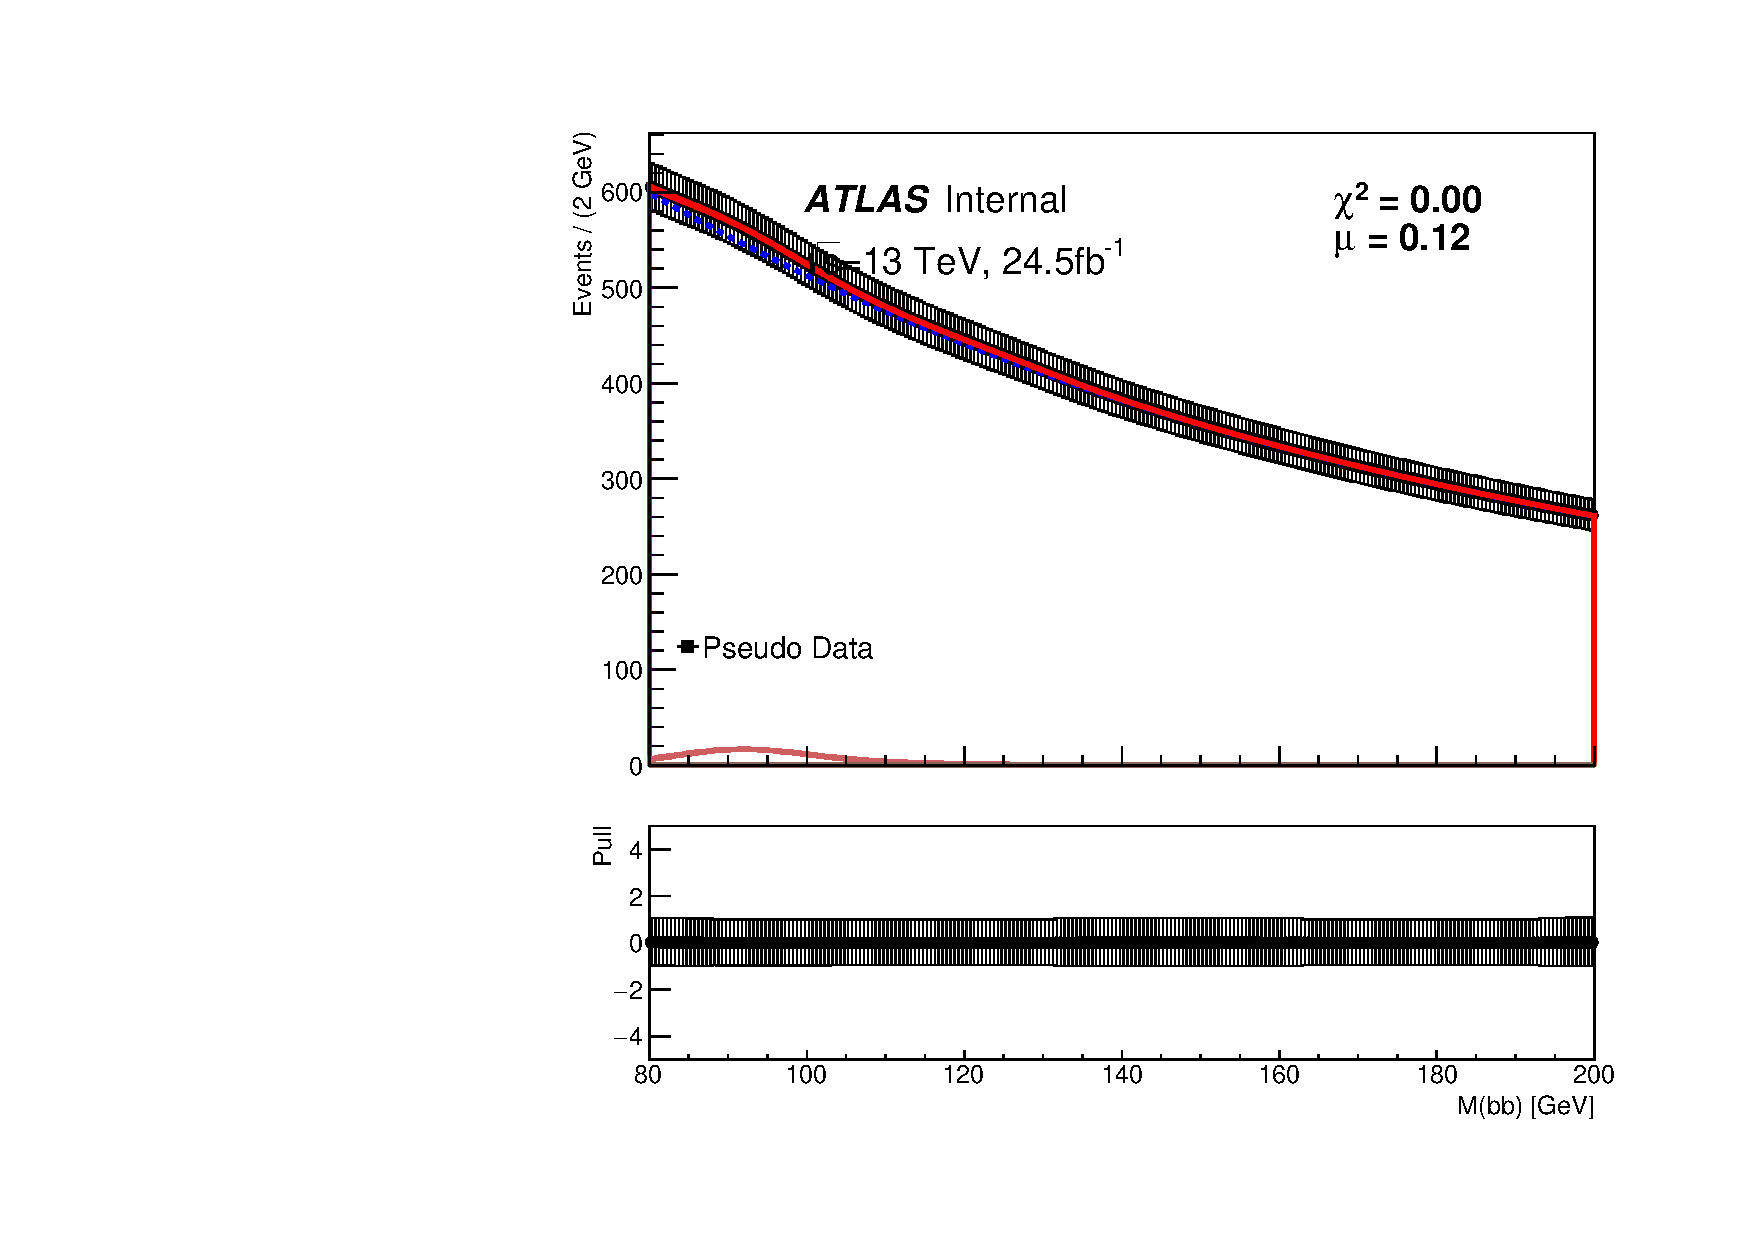
\includegraphics[width=0.24\textwidth]{figures/VBF/Spurious_ExpoO2_testVBF_ICHEP_2cen_SRI.pdf}
 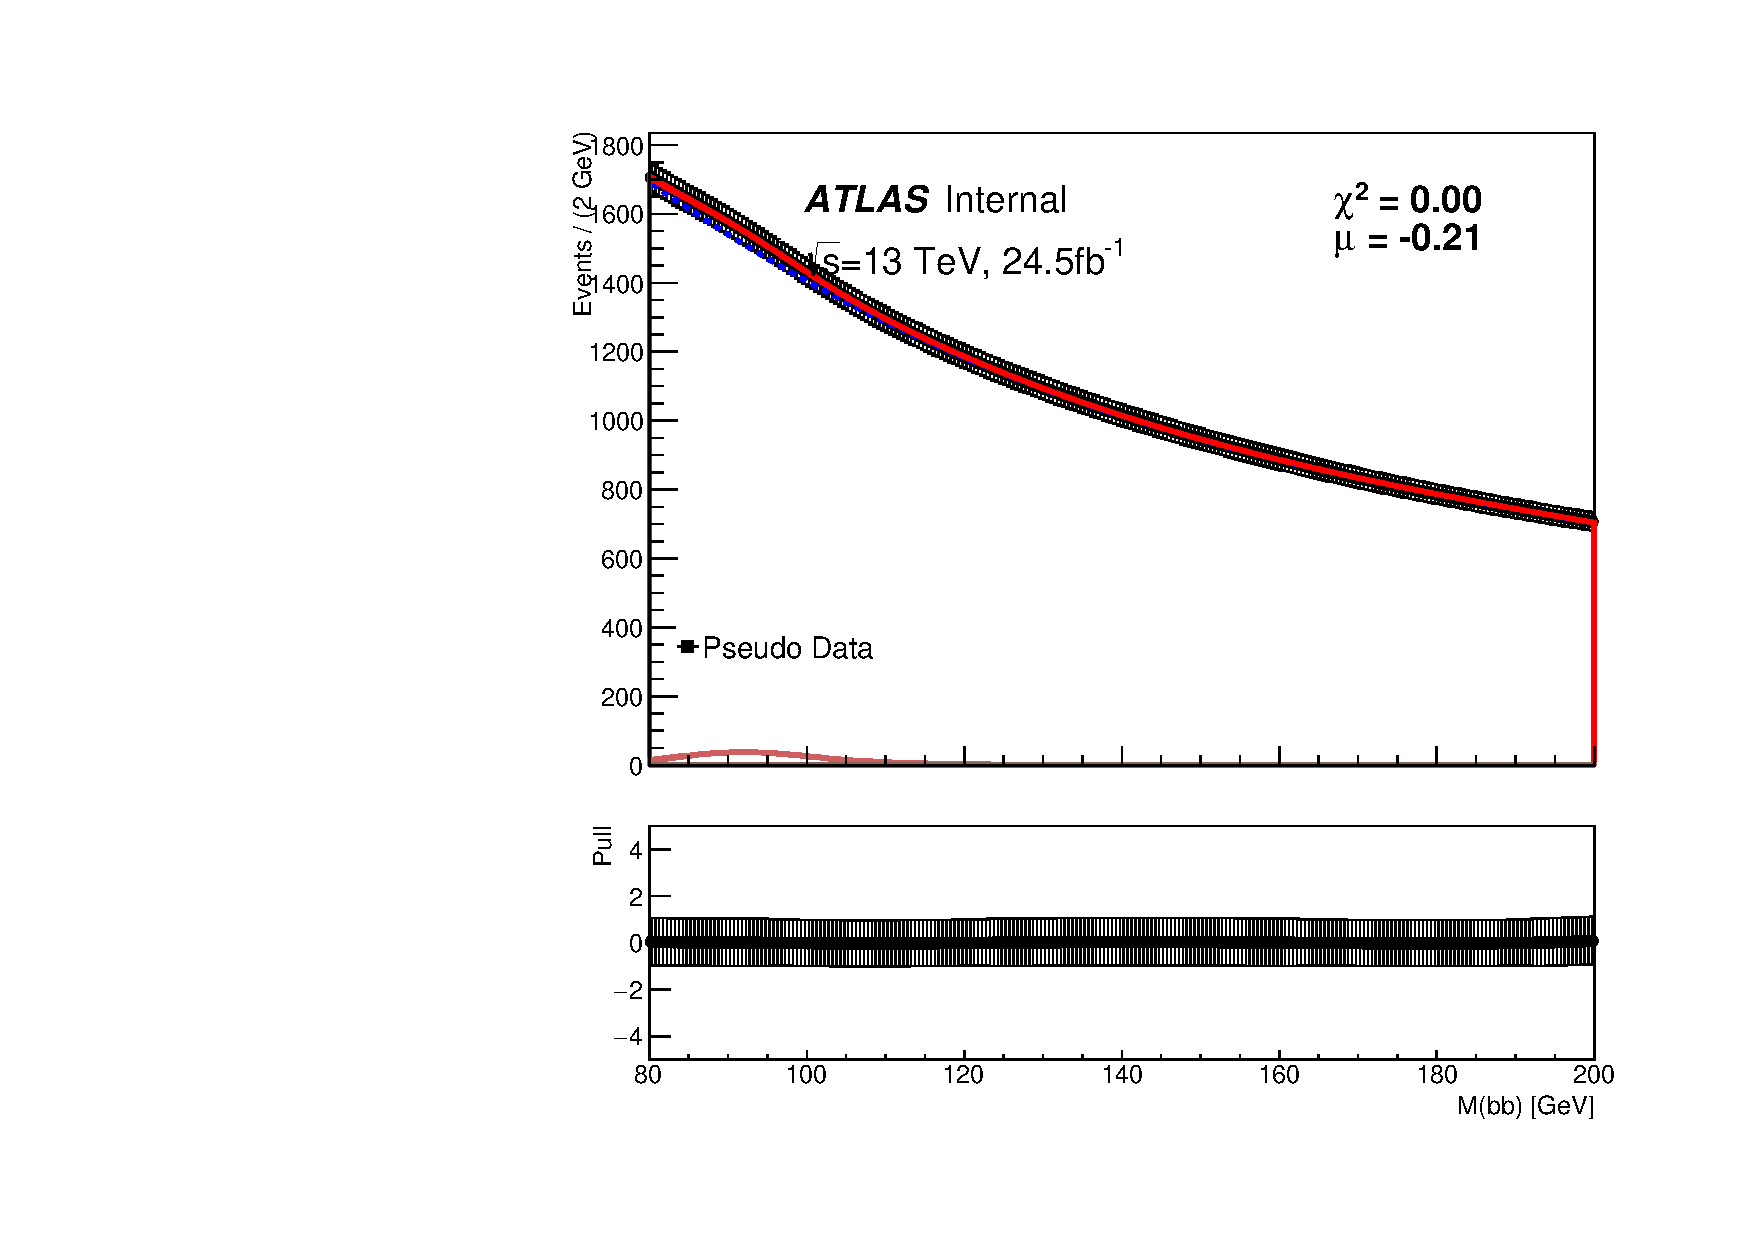
\includegraphics[width=0.24\textwidth]{figures/VBF/Spurious_ExpoO2_testVBF_ICHEP_2cen_SRII.pdf}\\
 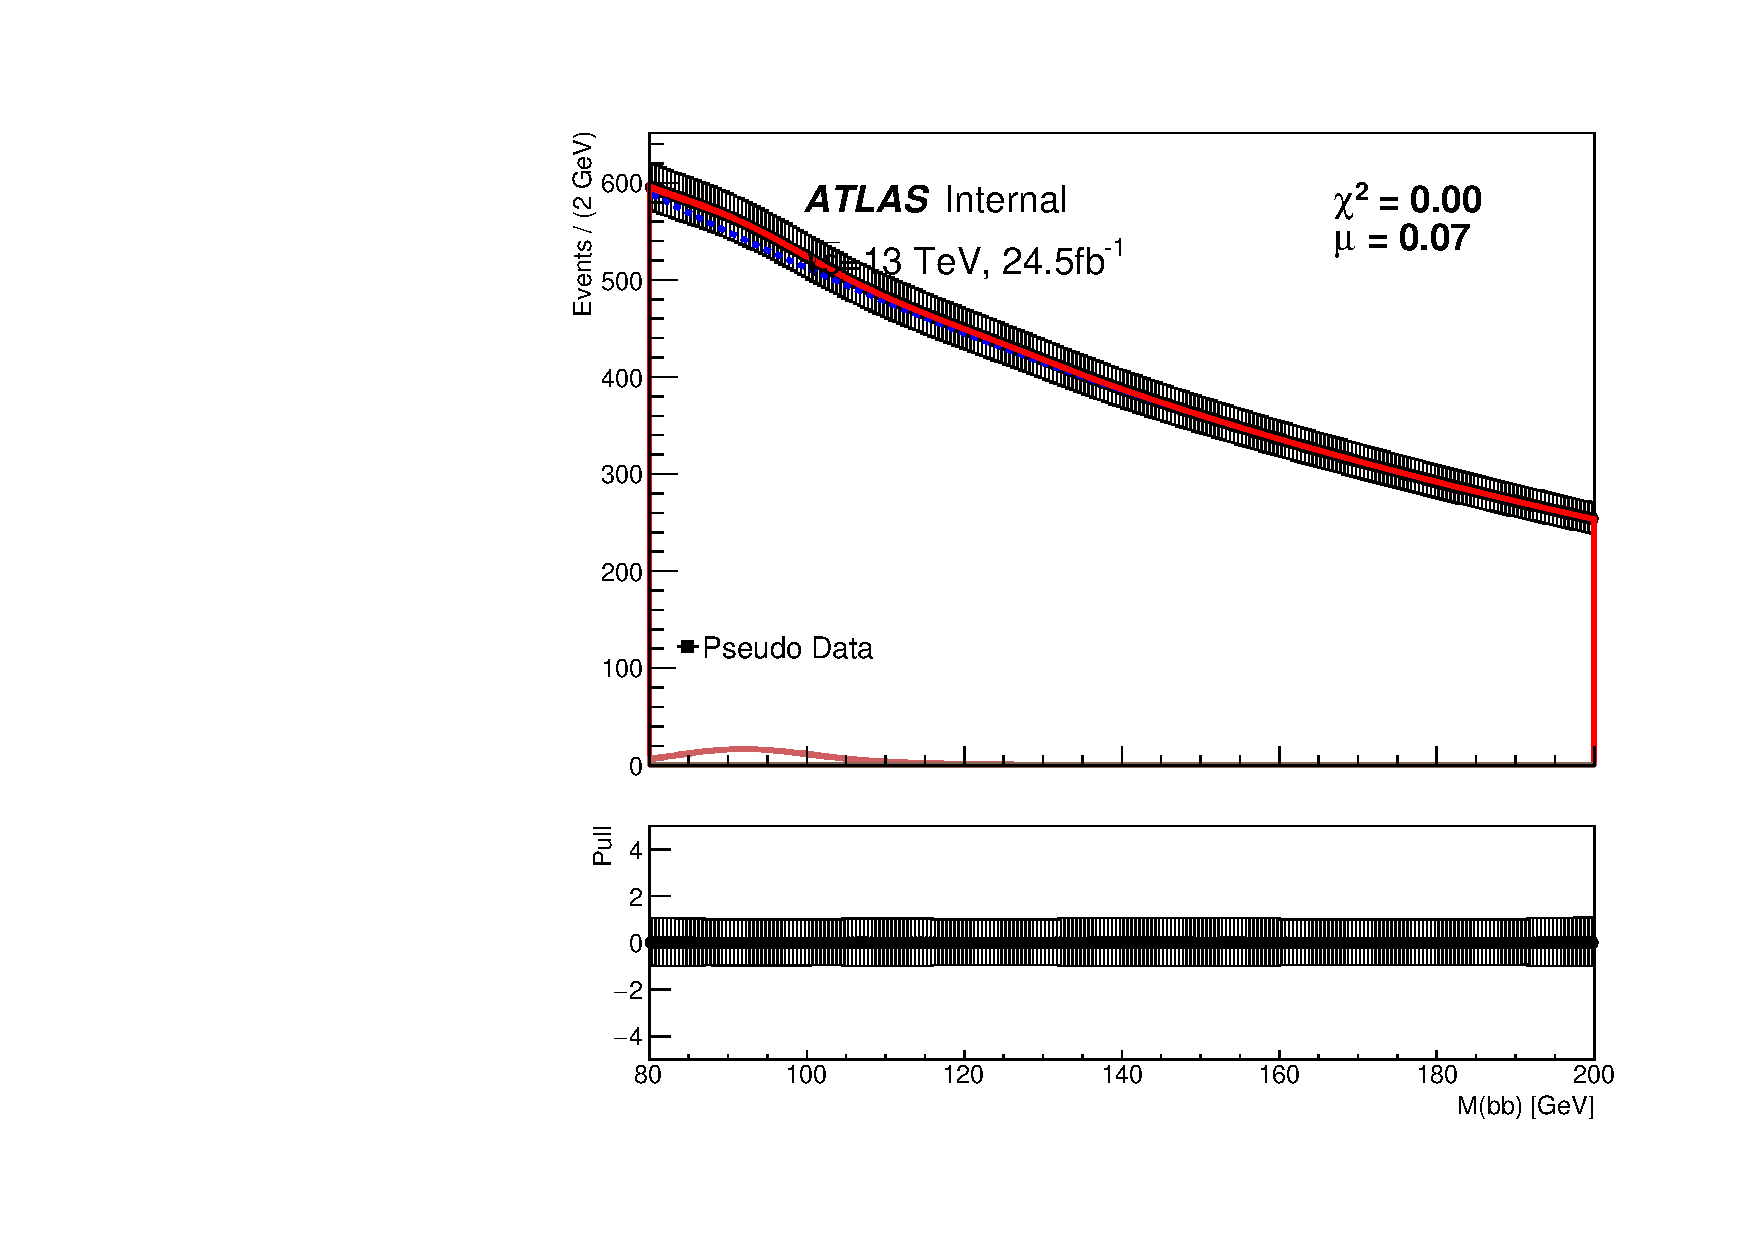
\includegraphics[width=0.24\textwidth]{figures/VBF/Spurious_SExpoO2_testVBF_ICHEP_2cen_SRI.pdf}
 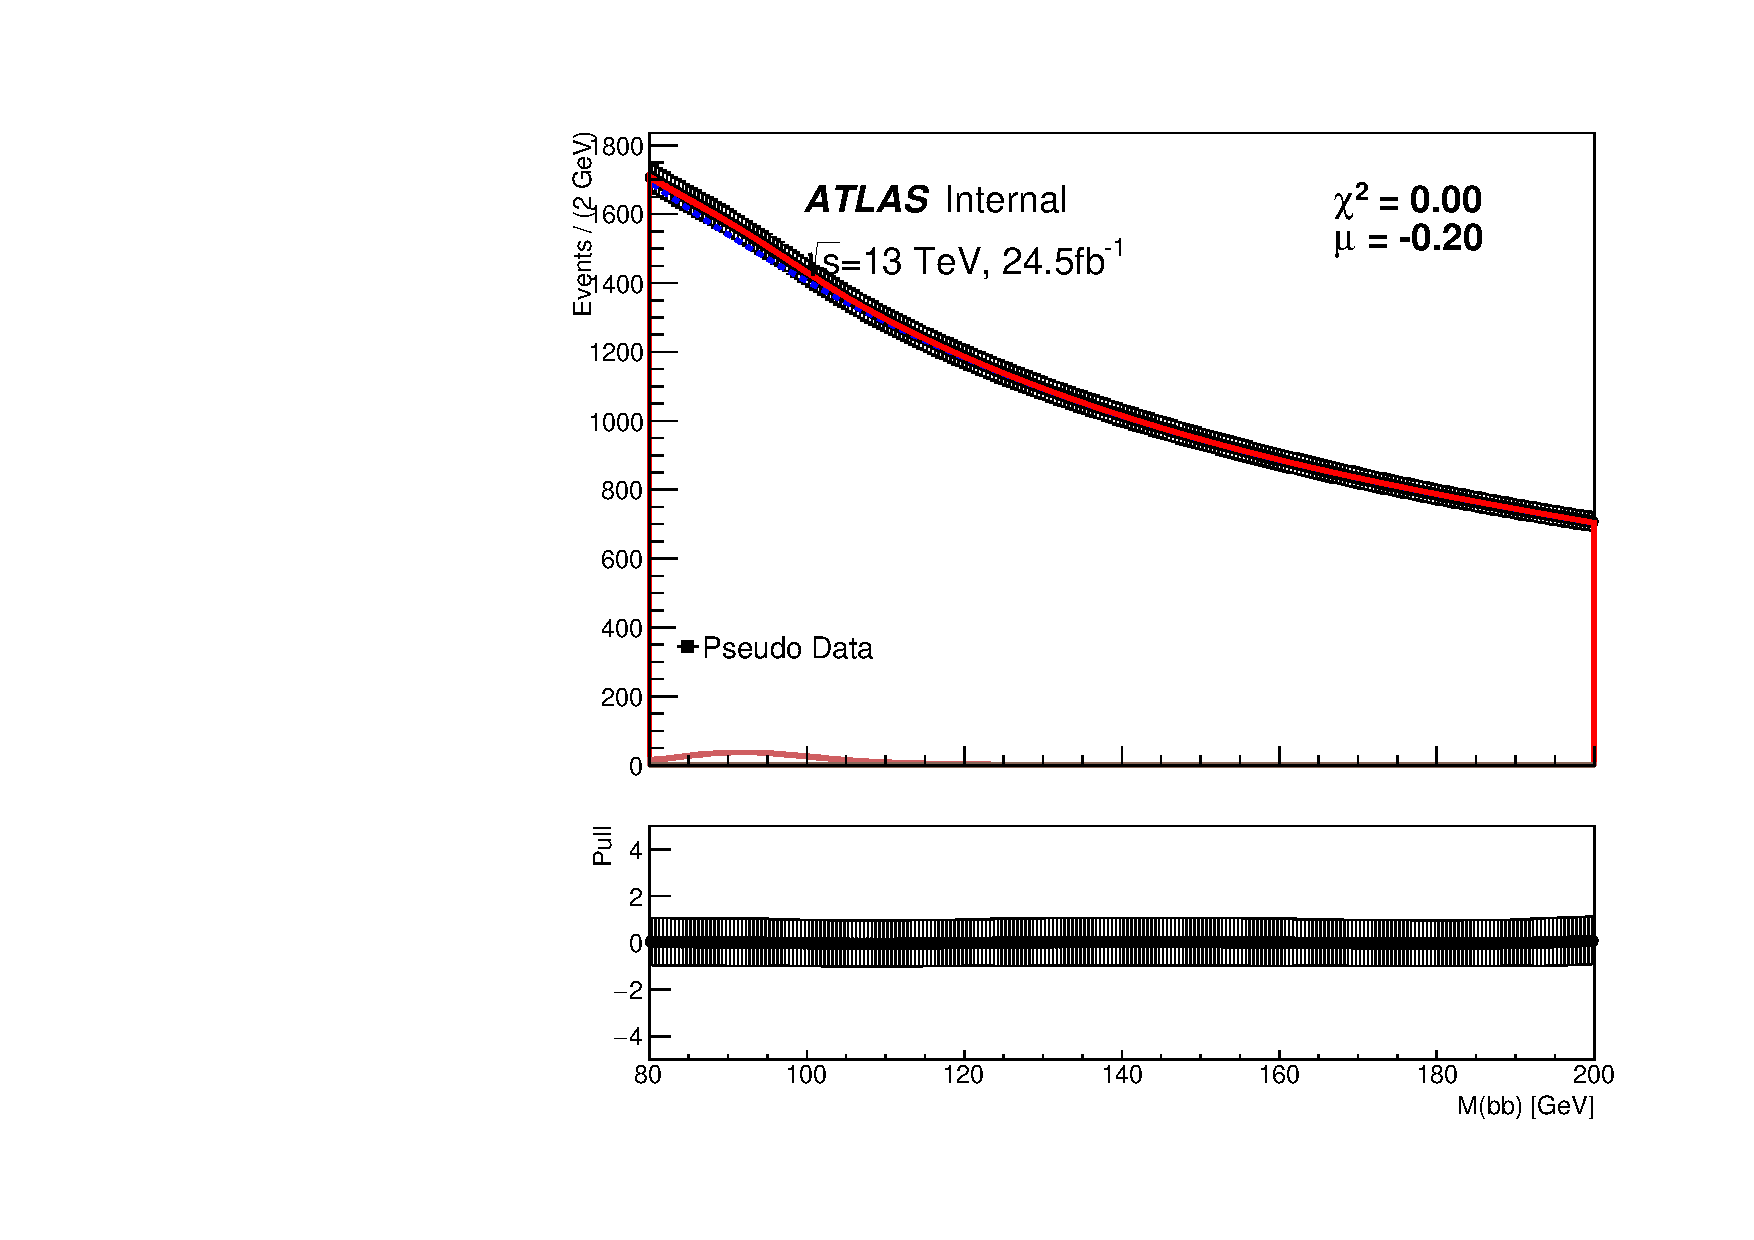
\includegraphics[width=0.24\textwidth]{figures/VBF/Spurious_SExpoO2_testVBF_ICHEP_2cen_SRII.pdf}\\
\caption{Spurious signal fit for \twocentral channel for SR I to SR II (from left to right). The best Bernstein background models are tested against alternative truth models Expo*Bernstein O(2) (top) and Sum of Expo O(2) (bottom).}
  \label{fig:vbf-Fit_SP_2cen}
\end{figure}

\begin{figure}[htbp]
  \centering
 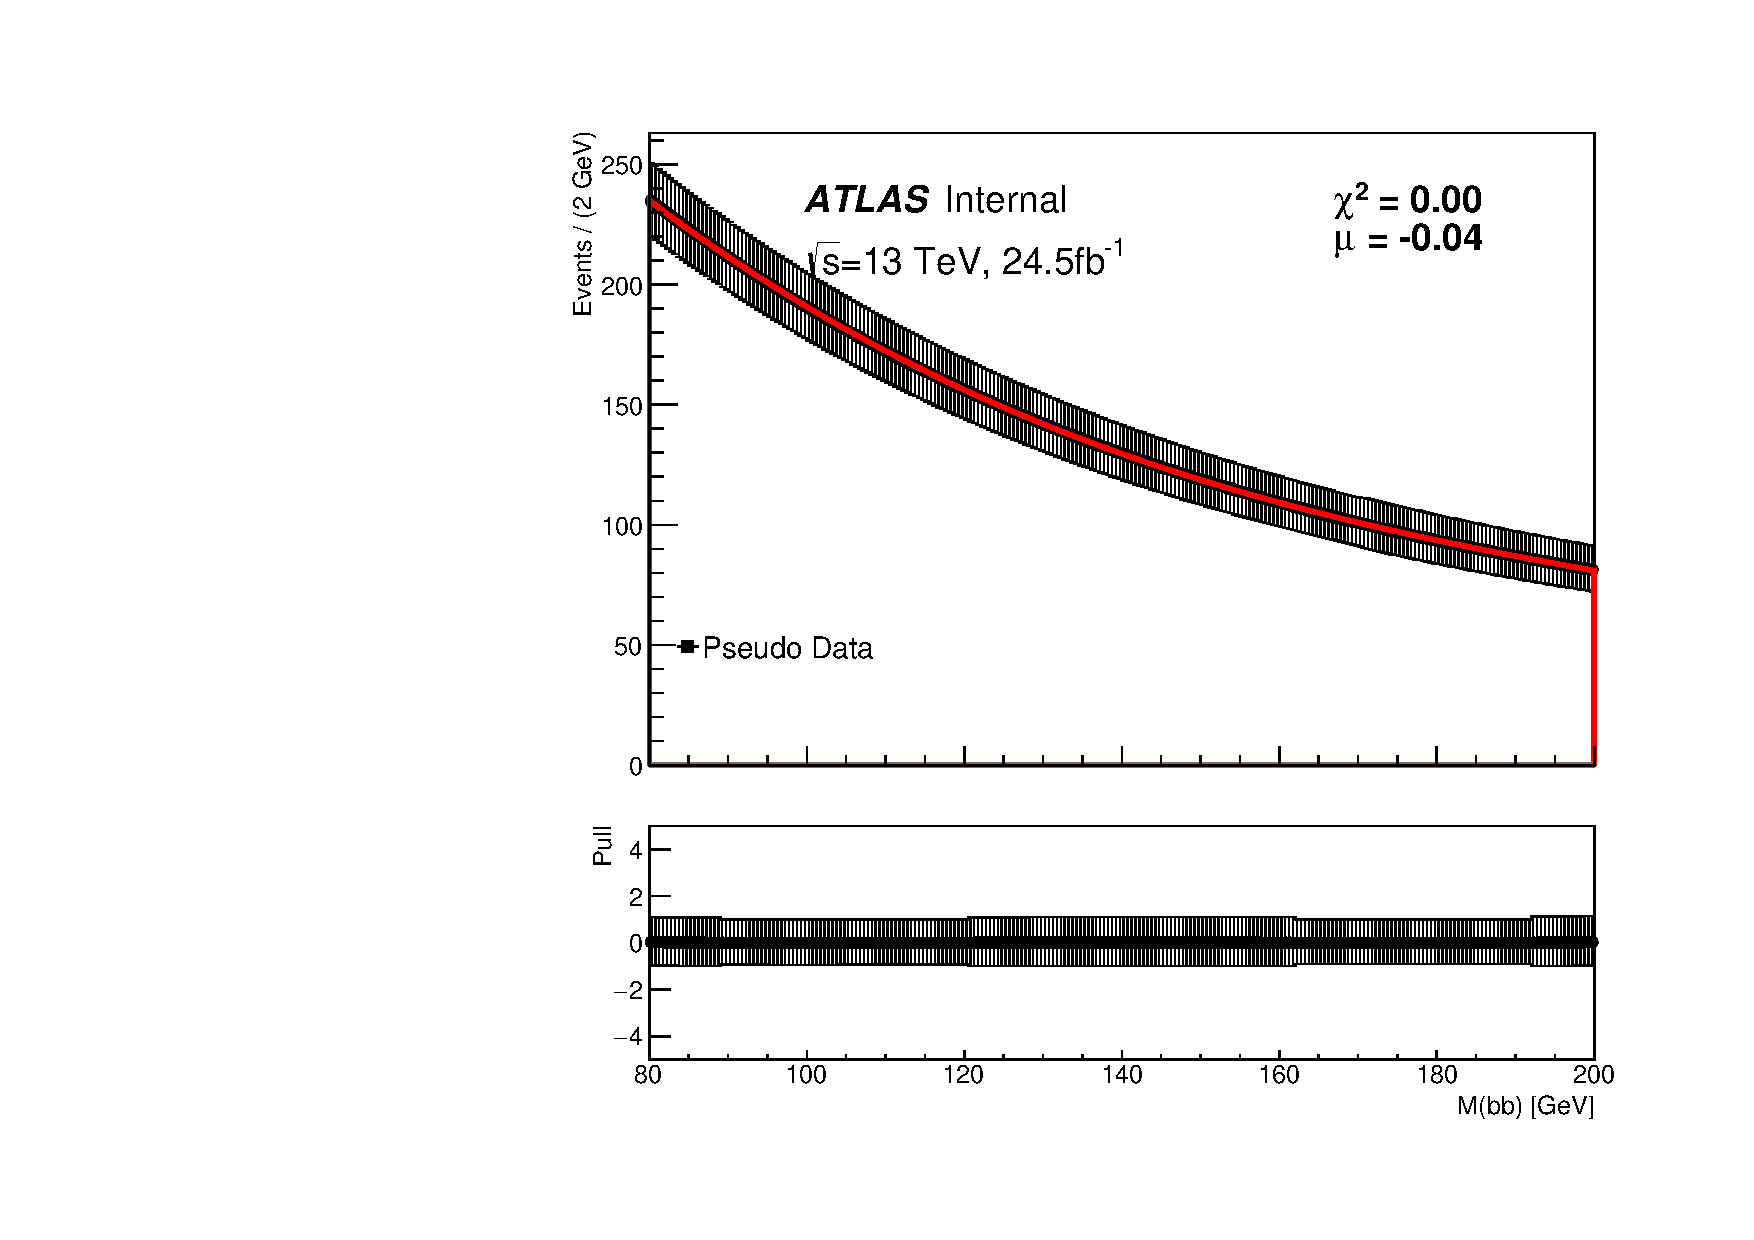
\includegraphics[width=0.24\textwidth]{figures/VBF/Spurious_ExpoO2_testVBF_ICHEP_4cen_SRI.pdf}
 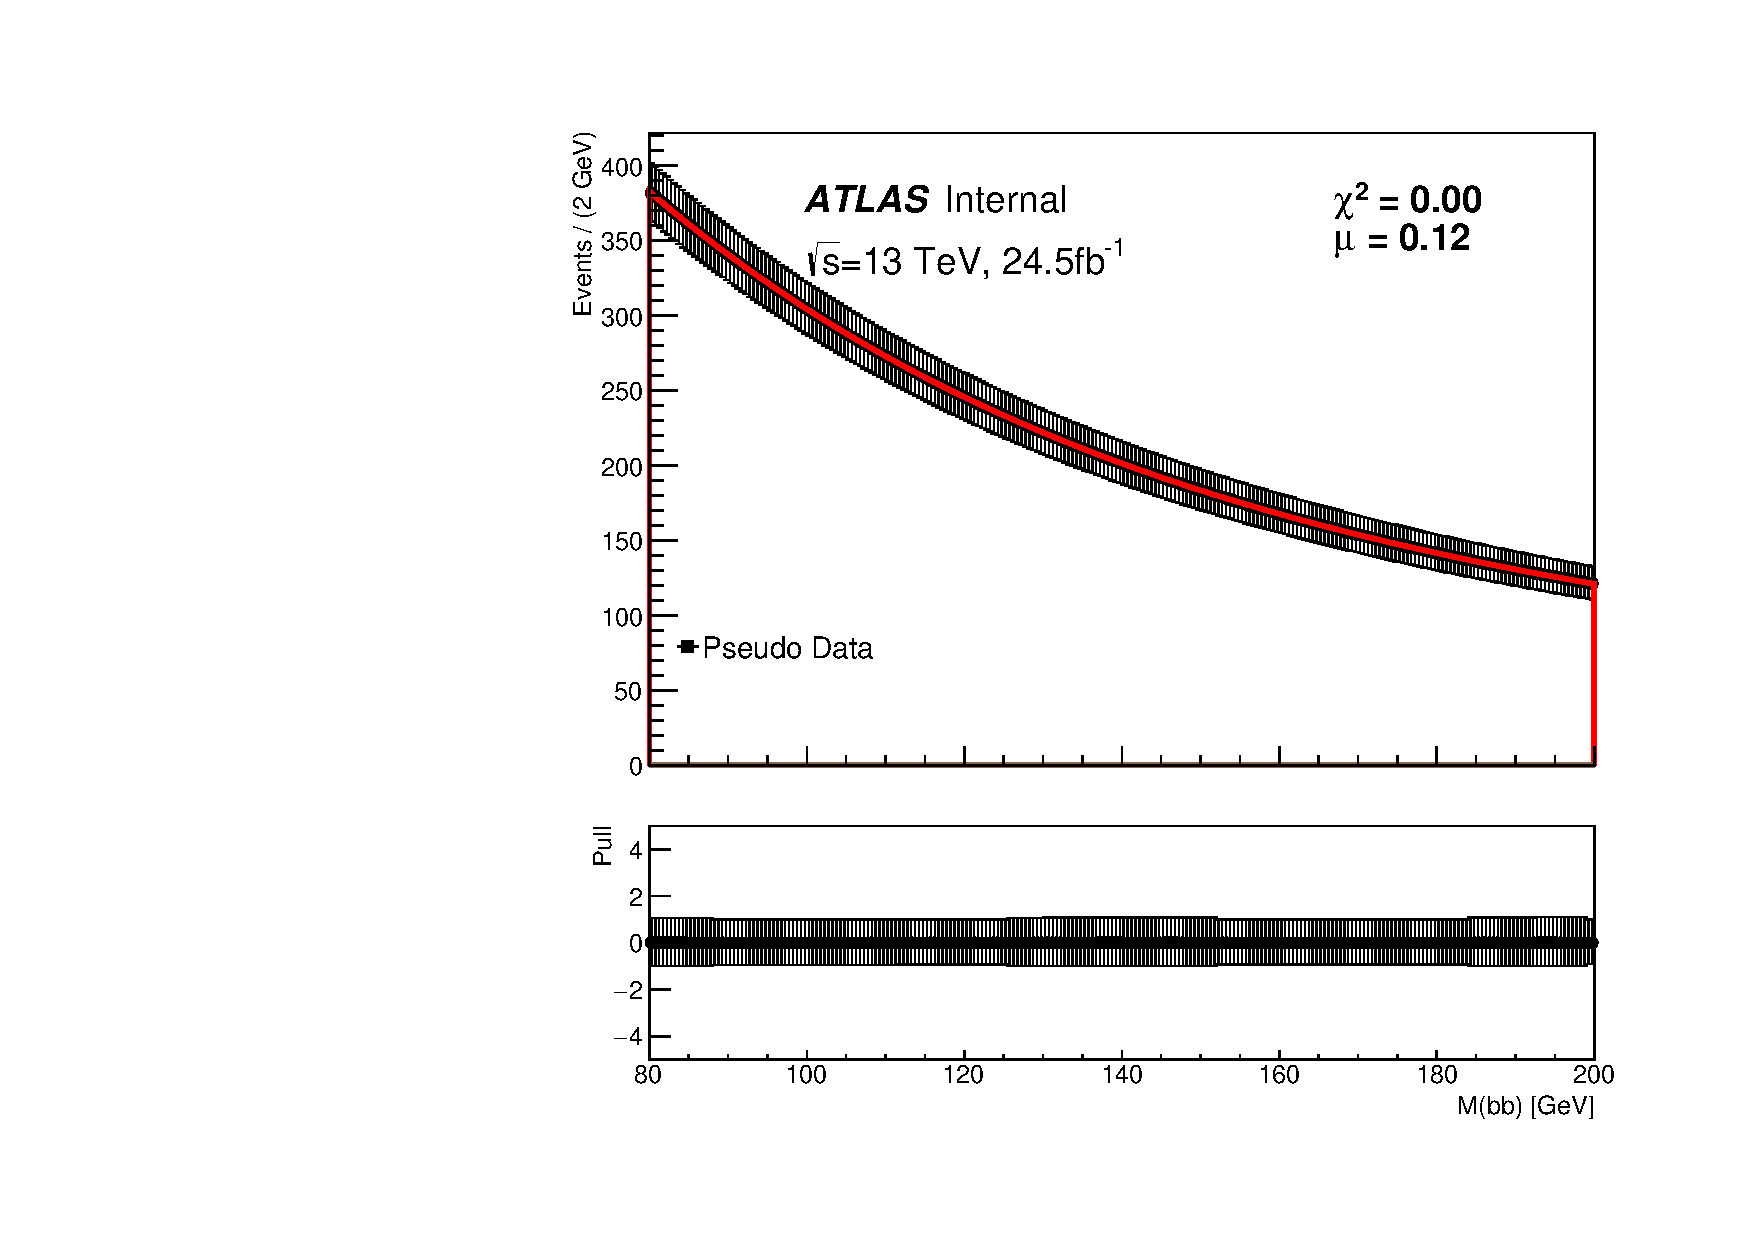
\includegraphics[width=0.24\textwidth]{figures/VBF/Spurious_ExpoO2_testVBF_ICHEP_4cen_SRII.pdf}
 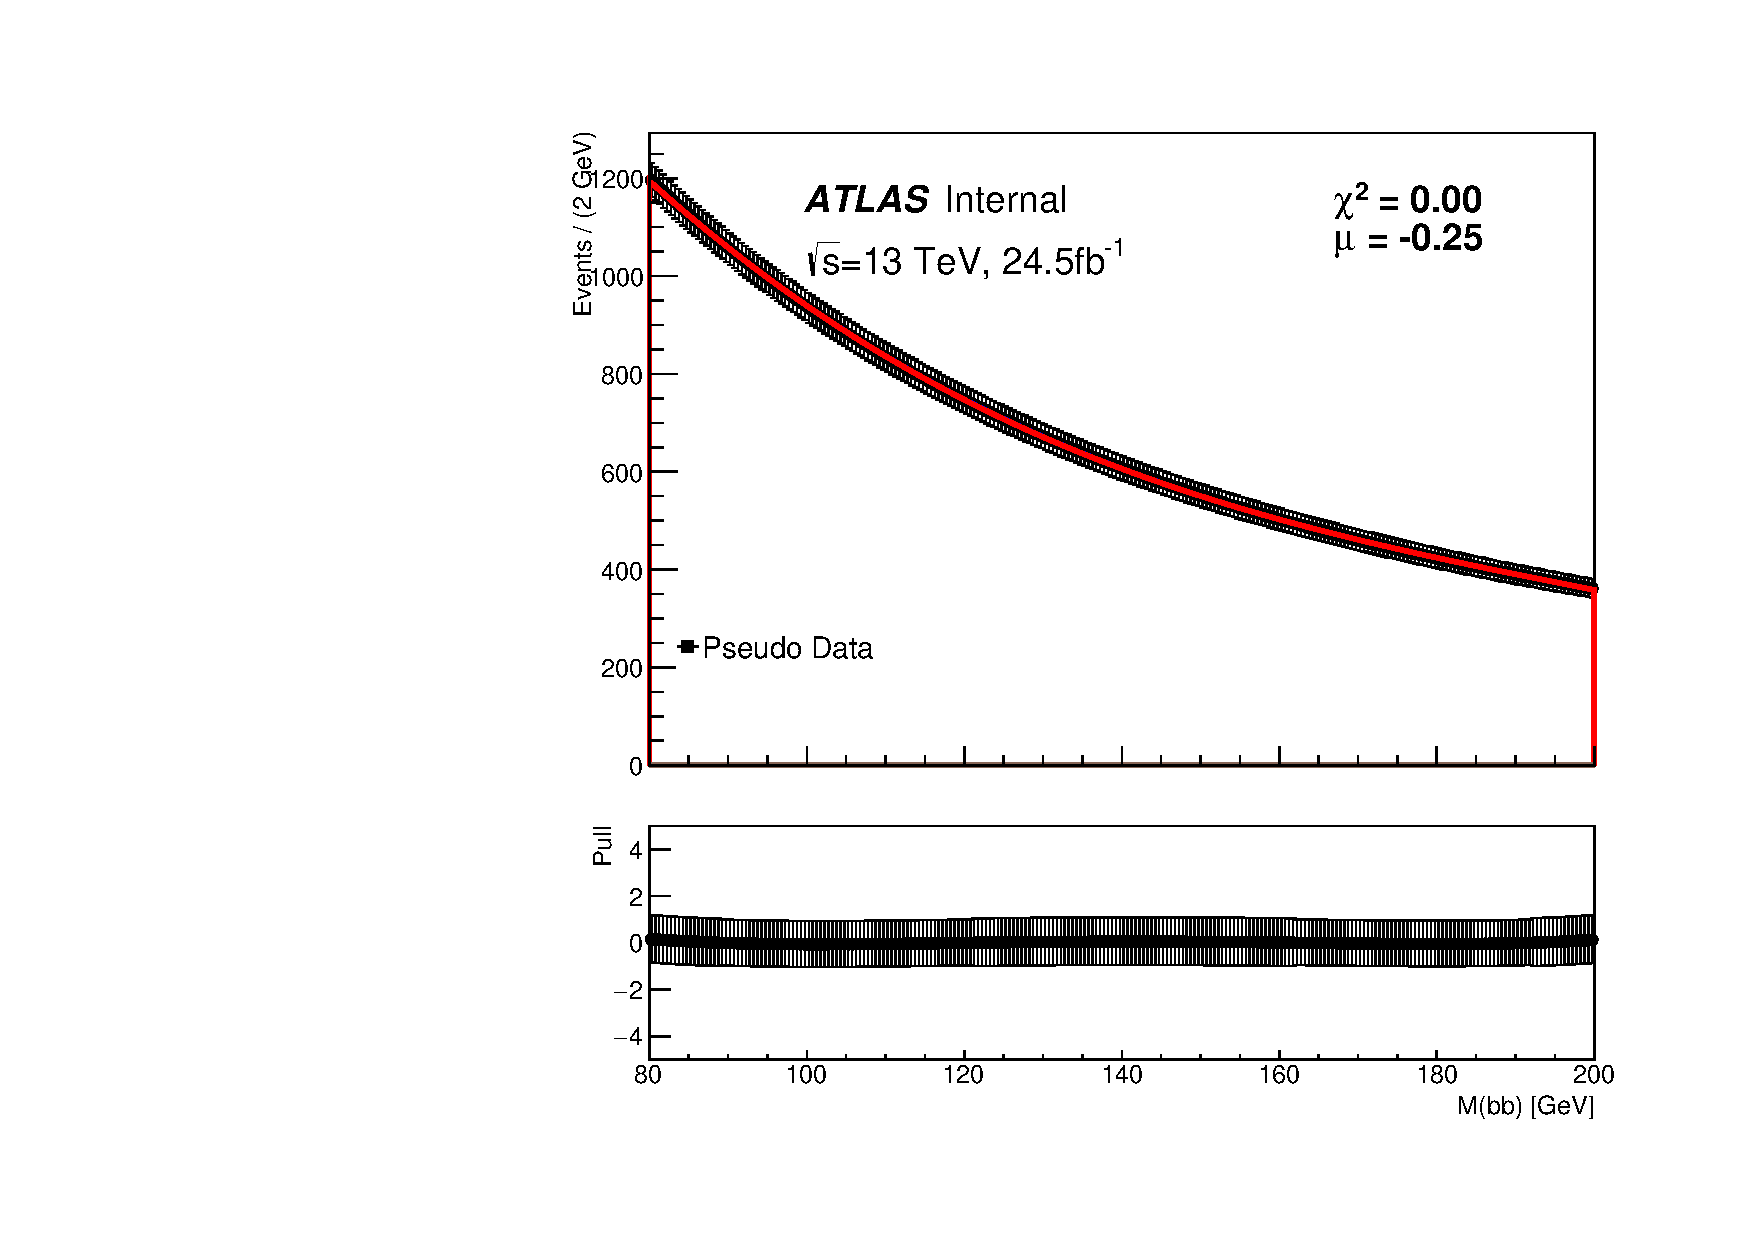
\includegraphics[width=0.24\textwidth]{figures/VBF/Spurious_ExpoO2_testVBF_ICHEP_4cen_SRIII.pdf}
 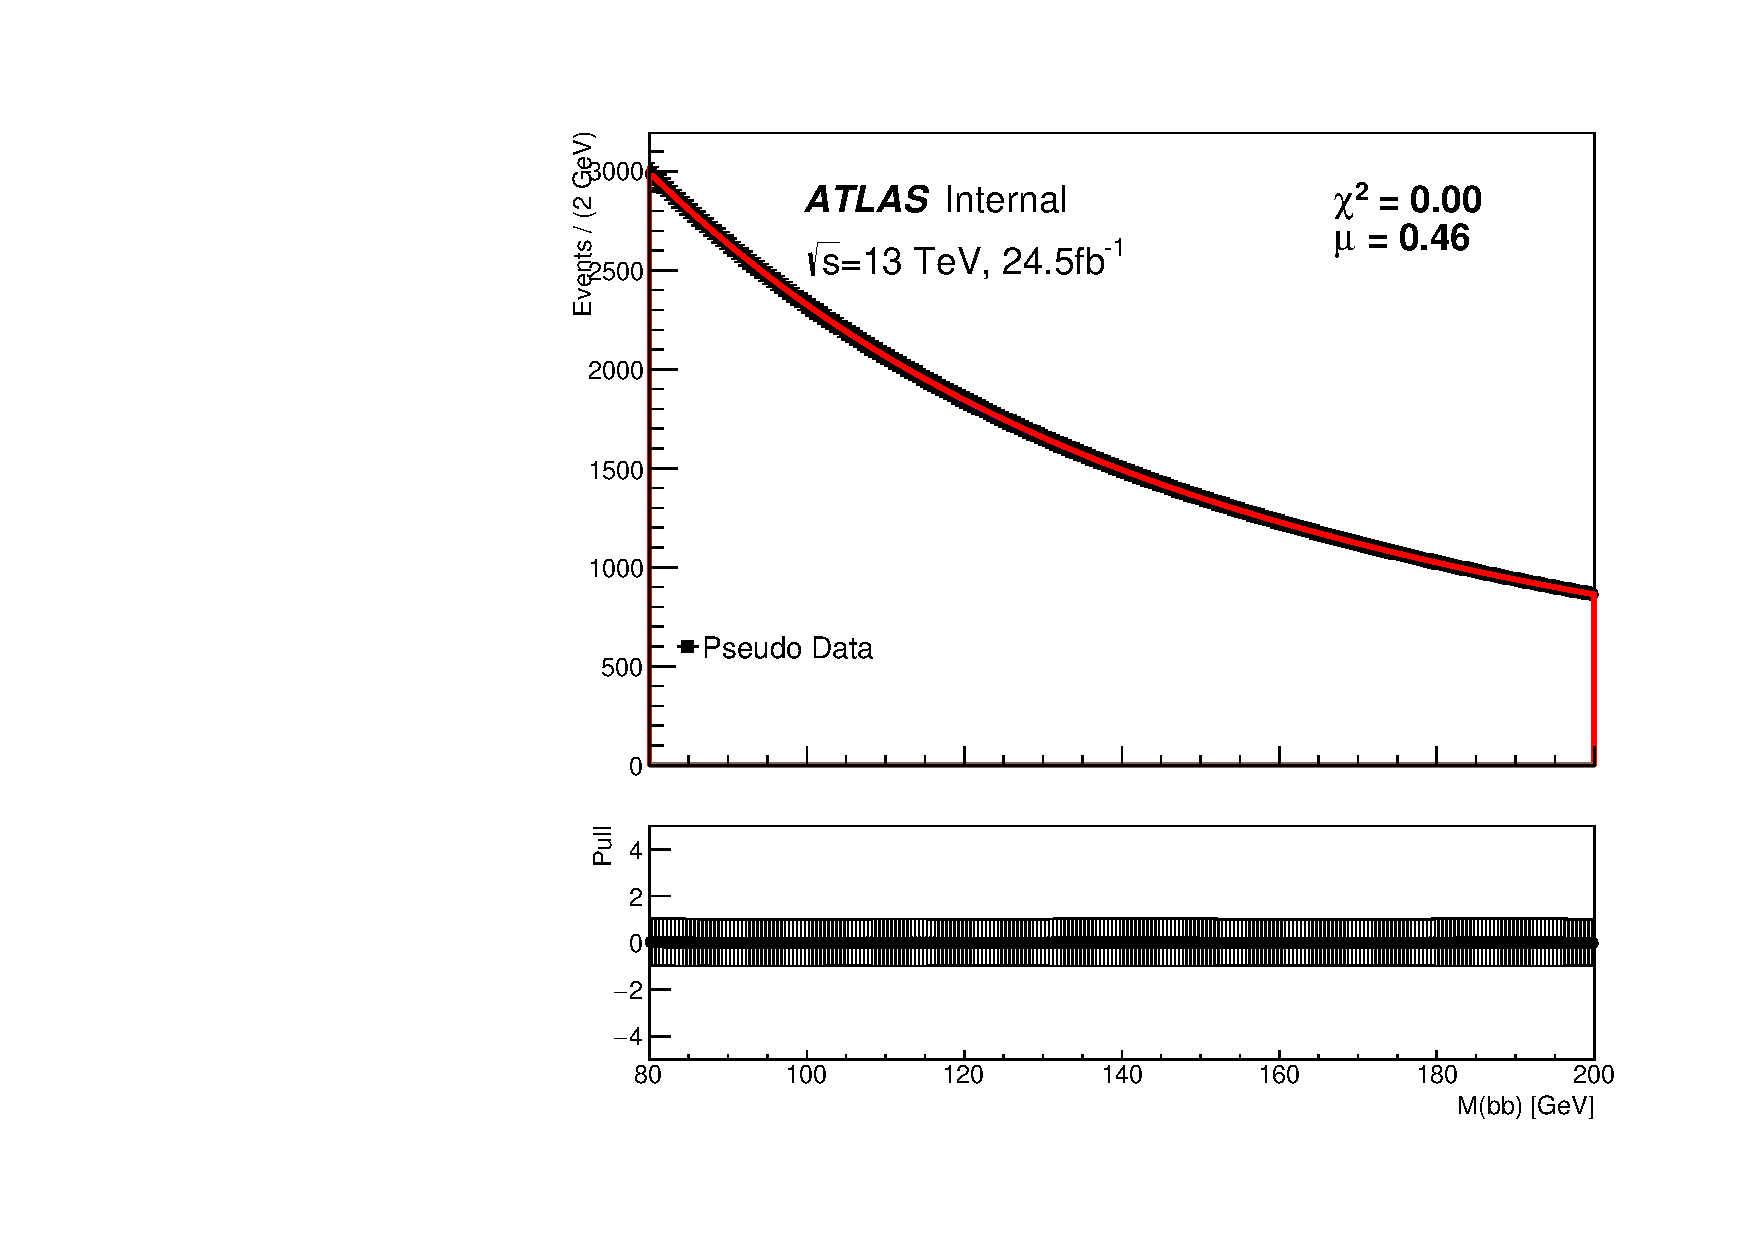
\includegraphics[width=0.24\textwidth]{figures/VBF/Spurious_ExpoO2_testVBF_ICHEP_4cen_SRIV.pdf}\\
 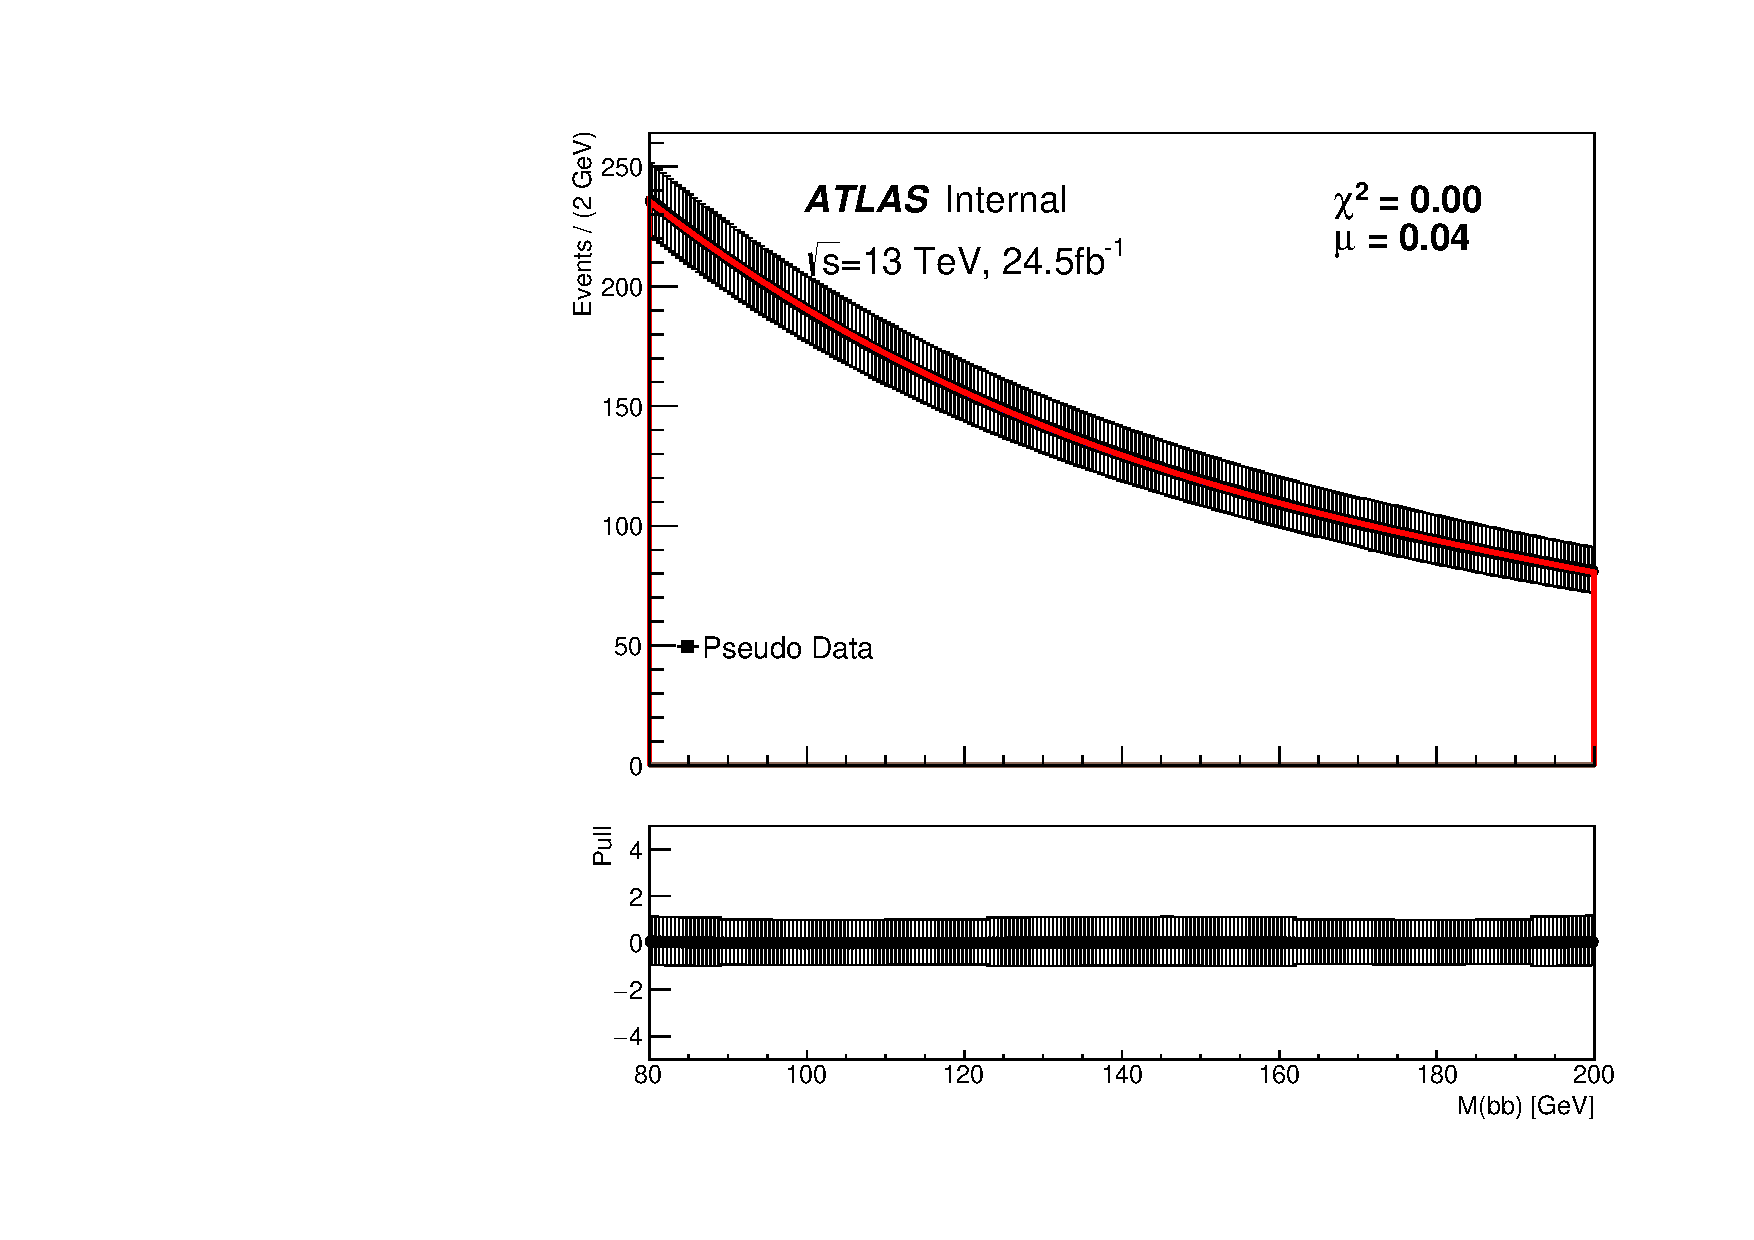
\includegraphics[width=0.24\textwidth]{figures/VBF/Spurious_SExpoO2_testVBF_ICHEP_4cen_SRI.pdf}
 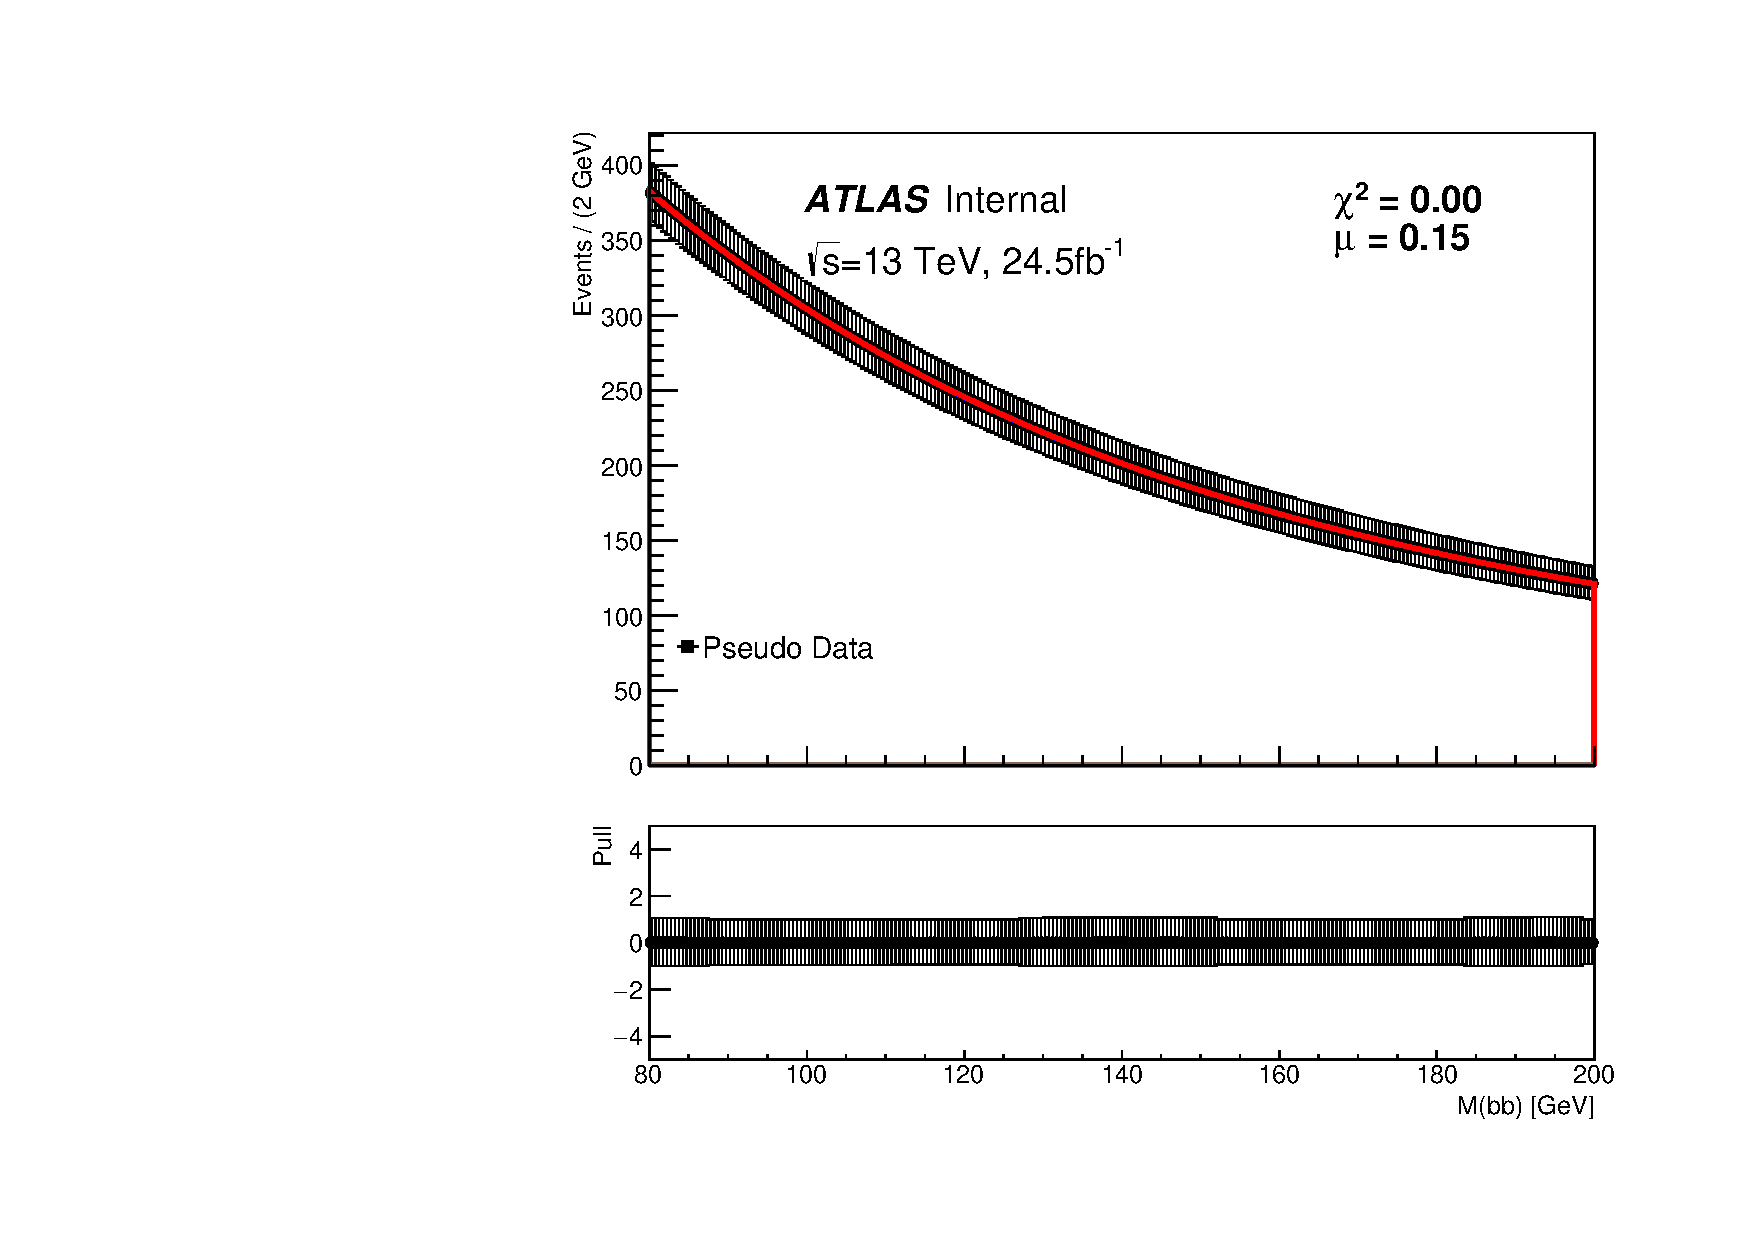
\includegraphics[width=0.24\textwidth]{figures/VBF/Spurious_SExpoO2_testVBF_ICHEP_4cen_SRII.pdf}
 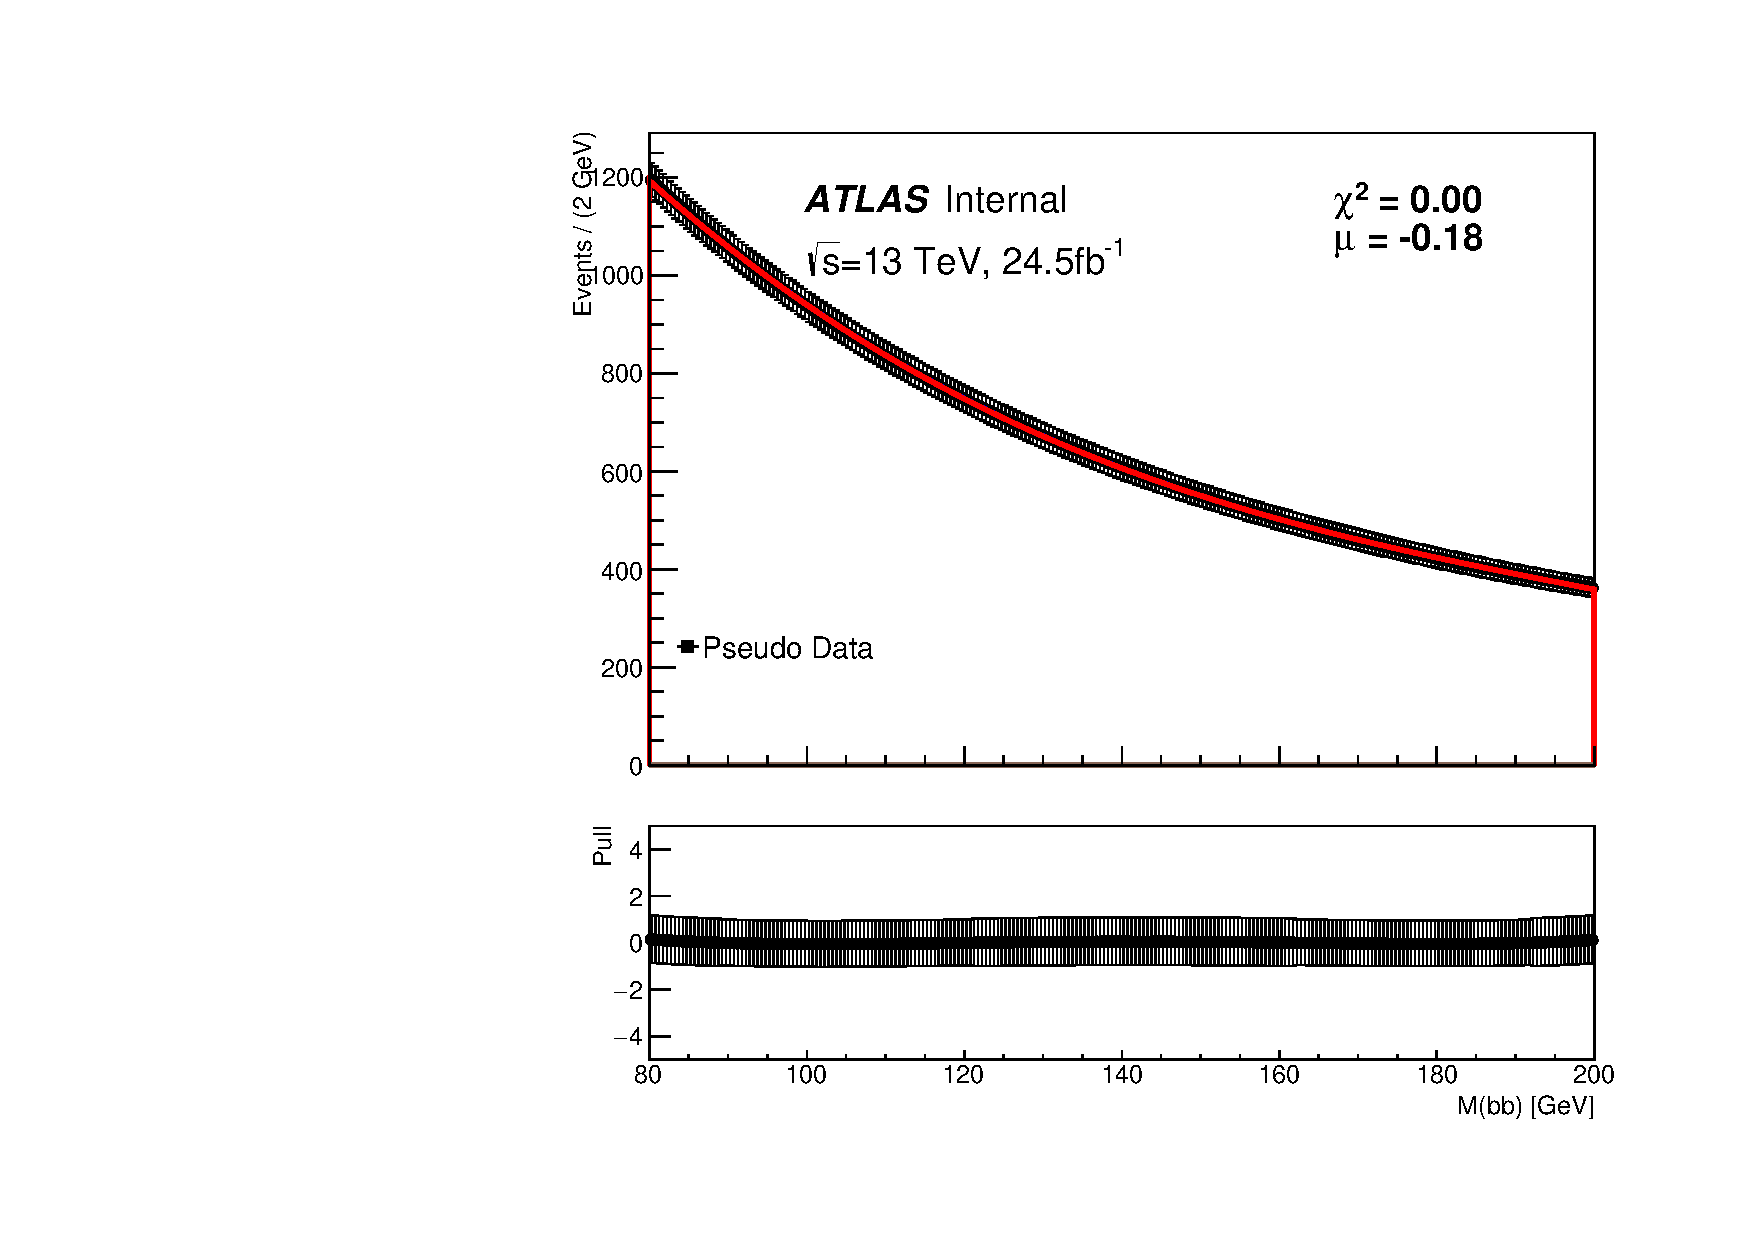
\includegraphics[width=0.24\textwidth]{figures/VBF/Spurious_SExpoO2_testVBF_ICHEP_4cen_SRIII.pdf}
 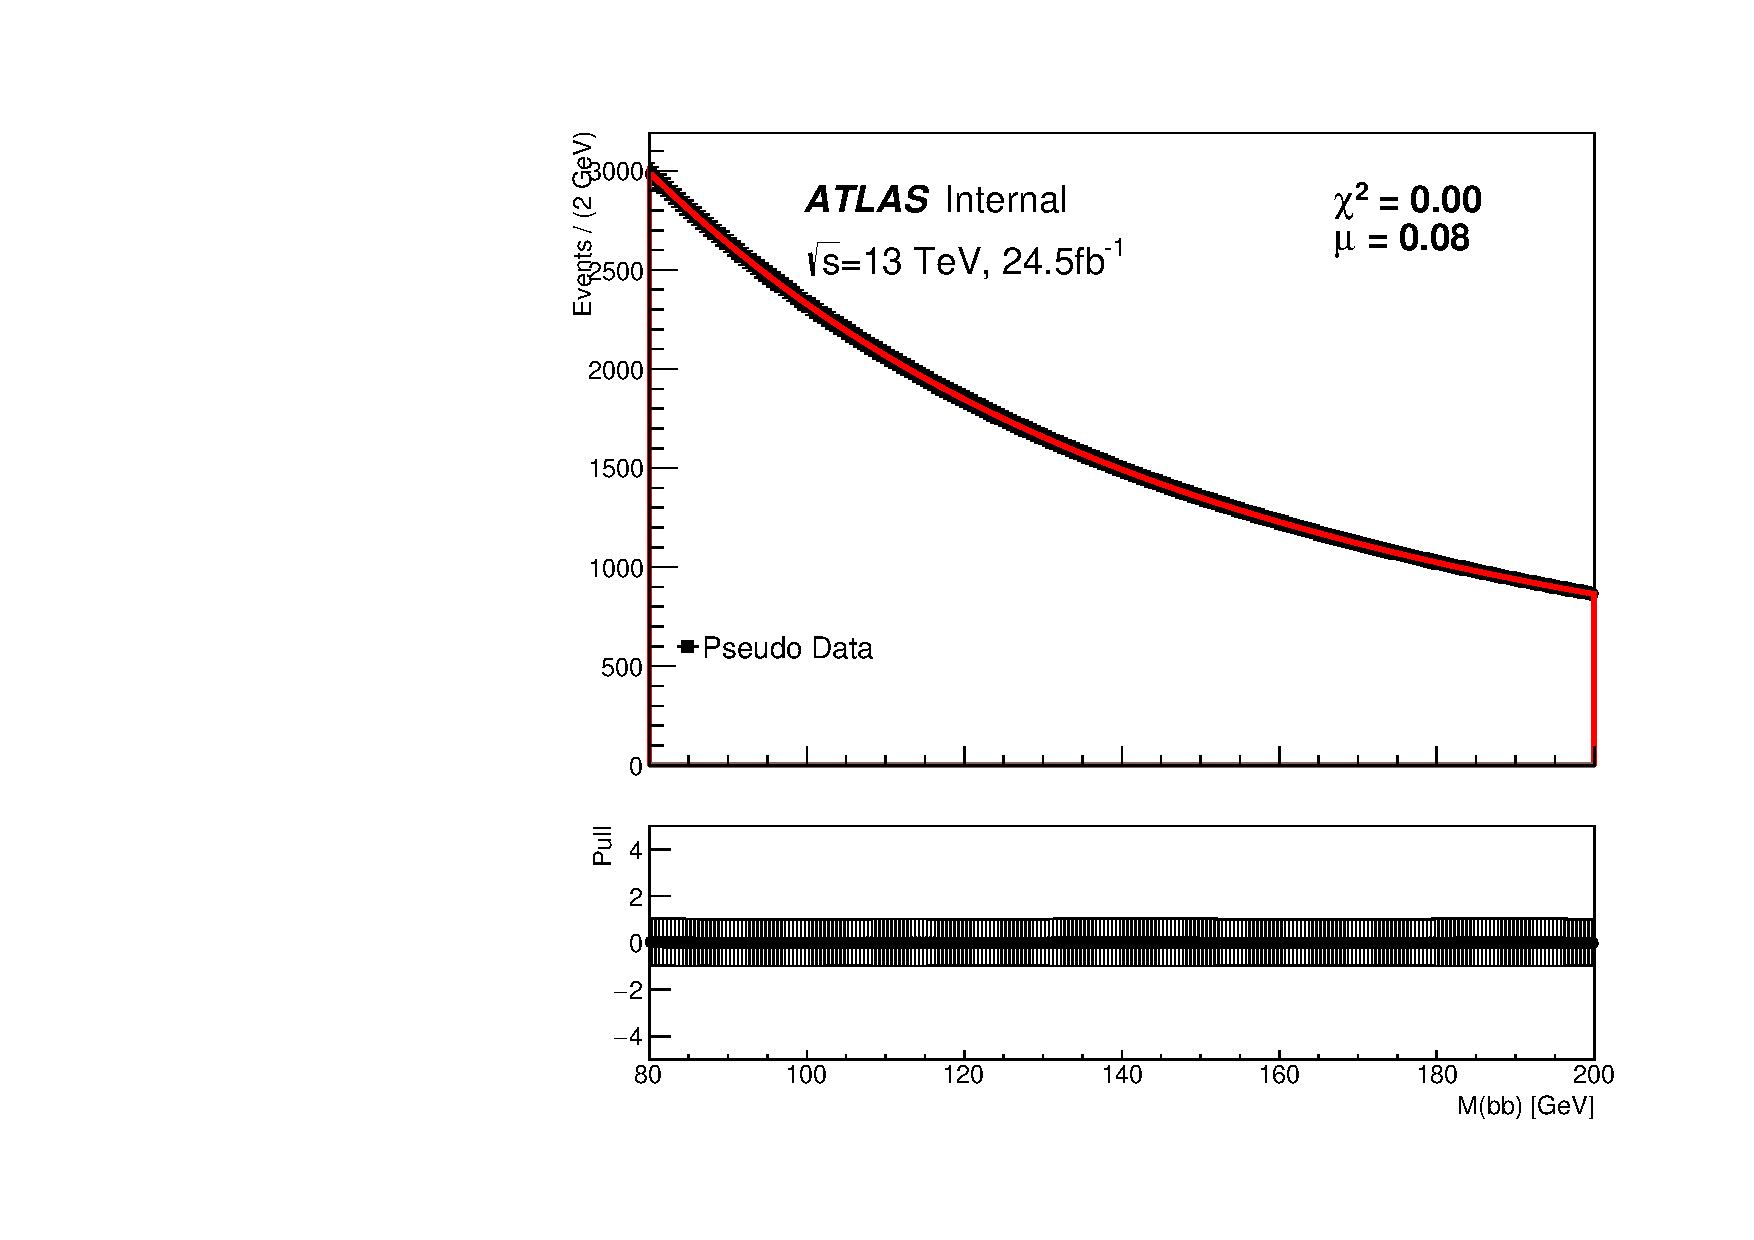
\includegraphics[width=0.24\textwidth]{figures/VBF/Spurious_SExpoO2_testVBF_ICHEP_4cen_SRIV.pdf}\\
\caption{Spurious signal fit for \fourcentral channel for SR I to SR IV (from left to right). The best Bernstein background models are tested against alternative truth models Expo*Bernstein O(2) (top) and Sum of Expo O(2) (bottom).}
  \label{fig:vbf-Fit_SP_4cen}
\end{figure}

